\chapter{Spatial Decomposition}{\label{ch:Spatial Decomposition}
  \def\figpath{chapters/SpatialDecomposition/figures/}
  \graphicspath{ {\figpath} }
  \newcommand{\resultwidth}{0.85\linewidth}
  %%%%%%%%%%%%%%%%%%%%%%%%%%%%%%%%%%%%%%%%%%%%%%%%%%%%%%%%%%%%%%%%%%%%%%%%%%%%%%
  % Introduction
  %%%%%%%%%%%%%%%%%%%%%%%%%%%%%%%%%%%%%%%%%%%%%%%%%%%%%%%%%%%%%%%%%%%%%%%%%%%%%%
  \section{Introduction}{\label{sec:Spatial Decomposition:Introduction}
    Until relatively recently, the method of choice for neutronics calculations has been neutron diffusion.
    Neutron diffusion codes can perform whole-core calculations, on a typical workstation, in relatively short run-times.
    However, with the recent shift towards higher fidelity methods such as \ac{SN}, and \ac{MOC} \cite{Askew1972}, more significant computational resources are necessary.
    These high fidelity methods allow for more detailed analysis, through finer resolution and use of fewer approximations, but typically take far more time to perform calculations; particularly for large calculations.
    Although processor clock-speeds have significantly improved, in the past several years computer cores have, for the most part, not gotten faster.
    To reduce the run-times (real-time) of high fidelity simulations, it is thus necessary to rely on parallelism.

    There are many different aspects of parallelism, and thread-based parallelism has been discussed previously \cref{sec:MOC:Parallelism}.
    Shared-data parallelism (threads), is limited to the resources of a single computational node.
    In order to utilize more resources, it is necessary to use a technique called \emph{domain decomposition}.
    Even without considerations for run-times, these high-fidelity simulations typically use more memory than is available on a single node, and domain decomposition becomes a necessity.
    In general, domain decomposition involves splitting up one domain of the problem into smaller subdomains; some typical domains to decompose are space, direction, and energy.
    Each smaller subdomain is assigned to a separate processor, and these can be run in parallel; although, there is generally some communication between the processors.

    In Monte-Carlo simulations, it is common that spatial decomposition involves duplication of some spatial locations.
    However, in deterministic transport methods, each domain is typically \emph{partitioned}, that is the domain is split without any overlap between subdomains.
    The MPACT \cite{MPACT2016} code has the ability to decompose two domains: space and direction.
    In MPACT, each discrete direction has a calculable amount of work, and the decomposition is trivial; in general, the same cannot be said of the spatial domain.
    This chapter focuses on improvements to the spatial decomposition techniques used in MPACT; these techniques, however, can be applied to other transport codes and similar results would be expected.
    The contents of this chapter are, in large part, adapted from an article published on this work \cite{Fitzgerald2019a}.

    As diffusion has been the method of choice for so long in the reactor physics field, spatial partitioning techniques common in other fields have, largely, not been applied.
    Transport codes such as MPACT \cite{MPACT2016}, or OpenMOC \cite{Gunow2018} used simple spatial partitioning methods that divided the core into uniformly sized blocks.
    However, the spatial partitioning of a reactor can be abstracted to a graph partitioning problem \cite{Fitzgerald2017}, which has been well studied in computer science \cite{Elsner1997} and applied to other simulation fields such as computational fluid dynamics \cite{Yao1998}.
    In general, the graph partitioning problem is \emph{NP-complete}, meaning that a partitioning cannot be easily verified as optimal; therefore, graph partitioning relies on approximate heuristic methods.
    Many different methods have been developed for graph partitioning, several of which are discussed in \cref{sec:Spatial Decomposition:Applied Graph Theory}.

    The remained of this chapter is structured as follows.
    In \cref{sec:Spatial Decomposition:Spatial Decomposition in MPACT}, a description of spatial decomposition in MPACT is given.
    \Cref{sec:Spatial Decomposition:Applied Graph Theory} introduces relevant graph theory concepts, and the methods used for spatial partitioning in this work.
    \Cref{sec:Spatial Decomposition:Applications for MPACT} describes the applications of these graph theory methods in MPACT.
    \Cref{sec:Spatial Decomposition:Results} compares methods for 2-D and 3-D reactor simulations.
    Finally, \cref{sec:Spatial Decomposition:Conclusions} lists the conclusions that are drawn from this work.
  }
  %%%%%%%%%%%%%%%%%%%%%%%%%%%%%%%%%%%%%%%%%%%%%%%%%%%%%%%%%%%%%%%%%%%%%%%%%%%%%%
  % Spatial Decomposition in MPACT
  %%%%%%%%%%%%%%%%%%%%%%%%%%%%%%%%%%%%%%%%%%%%%%%%%%%%%%%%%%%%%%%%%%%%%%%%%%%%%%
  \section{Spatial Decomposition in MPACT}{\label{sec:Spatial Decomposition:Spatial Decomposition in MPACT}
    The MPACT code uses the \ac{MOC} for neutronics calculations, and was originally developed for direct whole-core simulation of \acp{LWR}.
    As mentioned in \cref{ssec:RT:Modular Ray-Tracing}, MPACT uses the modular ray-tracing \cite{Saji2000} to significantly reduce track memory usage.
    The ray-tracing modules are small geometries that are often repeated in the reactor; these ray-tracing modules are used as the smallest unit for spatial decomposition in MPACT \cite{StimpsonPartitioning2017}.
    These ray-tracing modules are typically an axial slice of a quarter of a full fuel assembly, as shown in \cref{fig:Spatial Decomposition:5a-2d abstraction}
    The core consists of a structured grid of these modules in which each module has the same dimensions but may have different numbers of computational cells.
    Therefore, in MPACT, the spatial decomposition is a structured grid partitioning problem.

    In general, it is possible to use the computational cells as the smallest unit in the decomposition.
    However, this causes the decomposition problem to become an unstructured mesh partitioning problem.
    This has not been done in MPACT because communication would become significantly more complicated.
    Additionally, there would be more re-entrant rays which would have negative impacts on the rate of convergence.

    \begin{figure}
      \centering
      \begin{subfigure}[t]{0.45\textwidth}
        \centering
        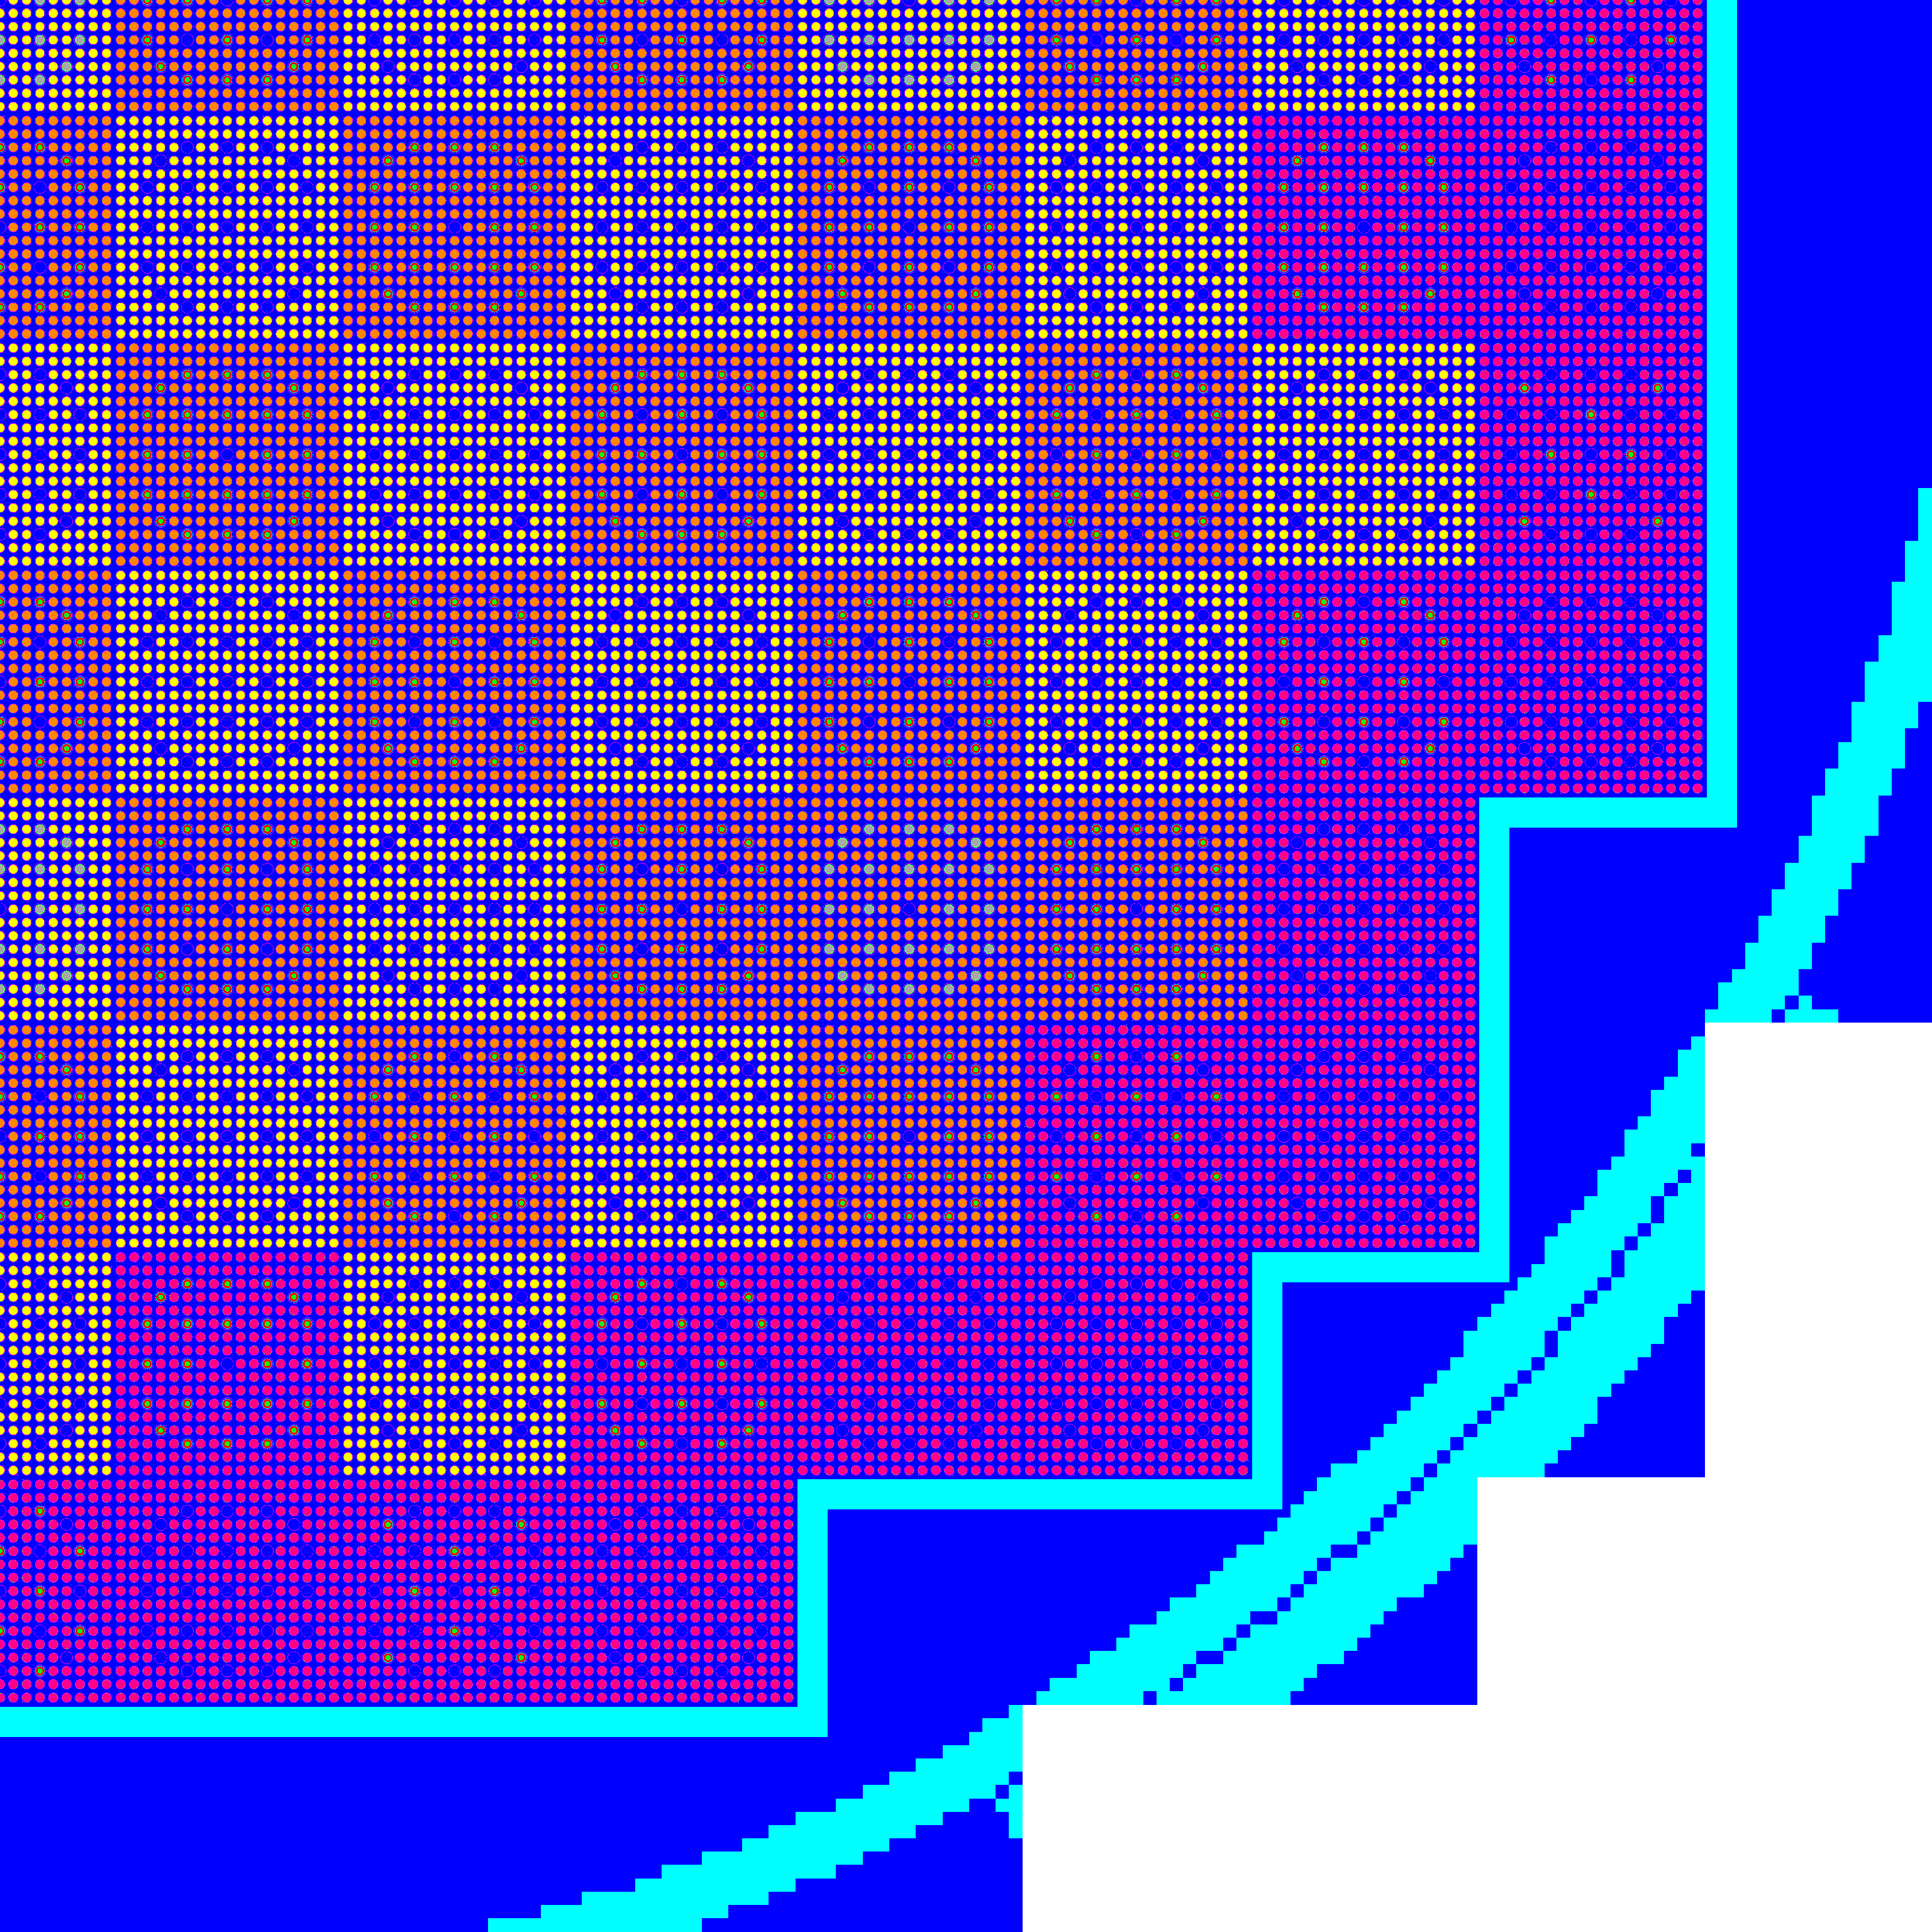
\includegraphics[width=0.9\textwidth]{5a-2d_core}
        \caption{fine mesh\label{fig:Spatial Decomposition:5a-2d configuration}}
      \end{subfigure}%
      ~
      \begin{subfigure}[t]{0.45\textwidth}
        \centering
        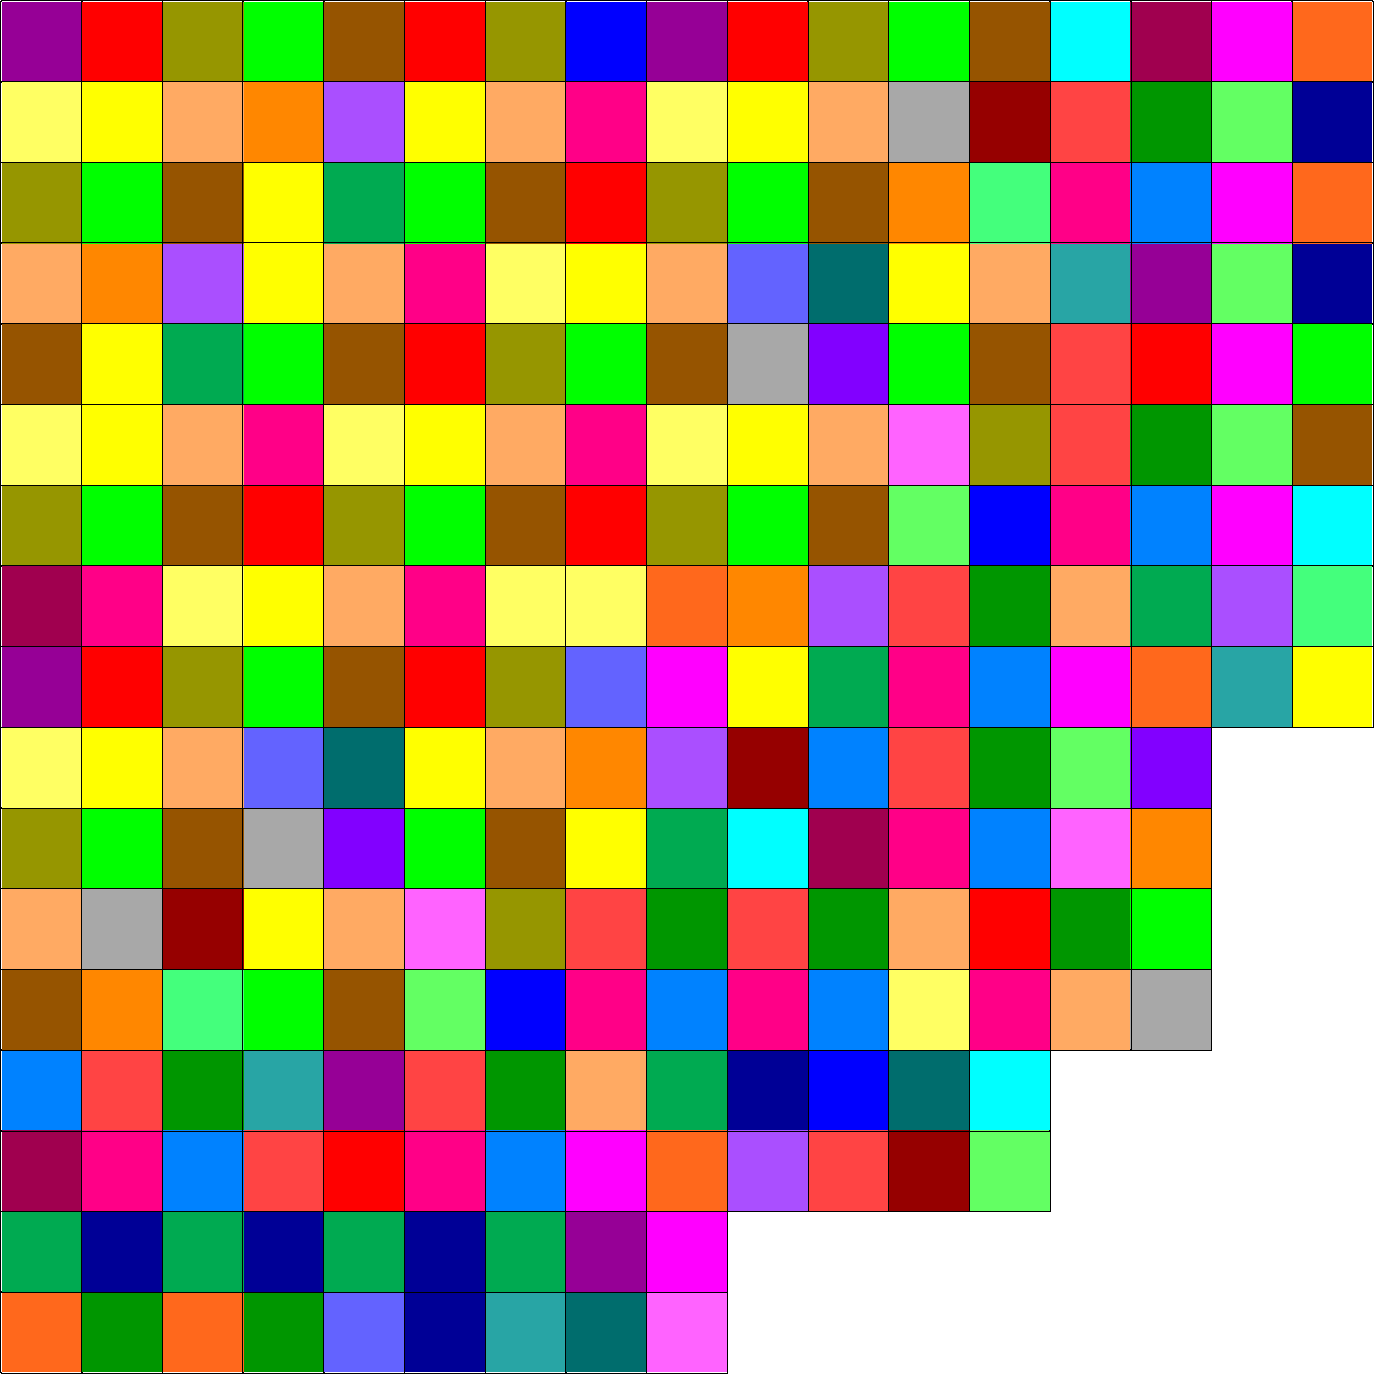
\includegraphics[width=0.9\textwidth]{modmesh_5a-2d}
        \caption{ray-tracing module mesh\label{fig:Spatial Decomposition:5a-2d modular mesh}}
      \end{subfigure}
      \caption{Example quarter core configuration and corresponding ray-tracing modular mesh in MPACT. \label{fig:Spatial Decomposition:5a-2d abstraction}}
    \end{figure}

    MPACT has had two spatial decomposition methods in the past: manual decomposition, and assembly-based decomposition.
    A user may manually enter a decomposition \cite{StimpsonPartitioning2017}, but it is time consuming to construct a balanced decomposition and will likely still be suboptimal to some degree.
    An automated method exists that recursively bisects the core using Morton-ordering \cite{Morton1966} applied to the reactor assembly geometries.
    While this method is automated, it often yields very imbalanced domains, and also restricts the number of subdomains that can be used.

    Previous work has shown that spatial decomposition of reactors can be abstracted to a graph partitioning problem \cite{Fitzgerald2017}.
    The use of graph partitioning methods in MPACT is expected to solve the issues encountered in each of the two approaches described above.
    These methods can be used to decompose into an arbitrary number of domains with high quality results, without user input.

    Existing graph partitioning libraries such as METIS \cite{METIS} partition graphs very efficiently and have very high quality results.
    To use all given processors, MPACT requires that each spatial subdomain contains at least one module, i.e. no partition can be empty.
    However, in some cases, particularly when the number of partitions is high, METIS may generate empty partitions.
    This means METIS cannot be used to decompose the core into an arbitrary number of subdomains without modifying the resulting partitions.
    For this reason, MPACT does not rely on third-party libraries for graph partitioning in the spatial decomposition process.
  }
  %%%%%%%%%%%%%%%%%%%%%%%%%%%%%%%%%%%%%%%%%%%%%%%%%%%%%%%%%%%%%%%%%%%%%%%%%%%%%%
  % Applied Graph Theory
  %%%%%%%%%%%%%%%%%%%%%%%%%%%%%%%%%%%%%%%%%%%%%%%%%%%%%%%%%%%%%%%%%%%%%%%%%%%%%%
  \section{Applied Graph Theory}{\label{sec:Spatial Decomposition:Applied Graph Theory}
    The spatial decomposition of a reactor core can be abstracted to the partitioning of a graph.
    Specifically, this would be a weighted graph, $G(V,E)$, which is comprised of a set of vertices, $V$, and a set of edges, $E$, that connect pairs of vertices.
    In general, these vertices and edges may have weights; a vertex $v_i$ will have weight $w_i$, and an edge $e_i$ between vertices $v_i$ and $v_j$ will have weight $c_{ij}$.
    In MPACT, a vertex represents a ray-tracing module, and the edges represent communication between adjacent modules in the \ac{MOC}.
    The graphs are undirected because communication between ray-tracing modules is two-way.

    Previous work \cite{Fitzgerald2017} applied unweighted graph partitioning techniques to the reactor spatial decomposition problem; the work presented here applies generalizations and improvements to the methods used for graphs with weighted vertices and edges.
    A vertex's weight indicates the amount of computational work that is needed; as one might expect, this is highly correlated with the number of computational cells.
    This is shown in \cref{sec:Spatial Decomposition:Results}.
    In general, the edges may also be weighted to account for different amounts of data transfer.
    This is discussed in more detail in \cref{sec:Spatial Decomposition:Applications for MPACT}.

    The goal is for each partition to have equal weight, with minimal weight of edges cut by partition boundaries.
    This is equivalent to each subdomain having the same amount of computational work with minimized communication between processes.
    If each process has roughly the same amount of work to perform, then less time will be spent waiting for other processes, thus improving parallel efficiency.
    Also, with less communication, less time will be spent passing data between processes, so the parallel overhead will be reduced.

    In this work, methods were separated into two distinct categories: partitioning methods and partition refinement (improvement) methods.
    Partitioning methods give a near-balanced partitioning for a given graph.
    Refinement methods attempt to reduce communication between existing partitions in a graph.
    As applied in MPACT, these refinement methods typically did not significantly reduce communication.
    These methods and results are presented in \cref{sec:Spatial Decomposition:Partition Refinement}.
    %%%%%%%%%%%%%%%%%%%%%%%%%%%%%%%%%%%%%%%%%%%%%%%%%%%%%%%%%%%%%%%%%%%%%%%%%%%%
    % Graph Partitioning Methods
    %%%%%%%%%%%%%%%%%%%%%%%%%%%%%%%%%%%%%%%%%%%%%%%%%%%%%%%%%%%%%%%%%%%%%%%%%%%%
    \subsection{Graph Partitioning Methods}{\label{ssec:Spatial Decomposition:Graph Partitioning Methods}
      In this work, recursive partition methods were considered due to their capability to partition into arbitrary numbers of domains.
      Each of these recursive partitioning methods sorts the graph, using different methods, and then divides or ``cuts'' the graph into two sub-graphs with approximately equal vertex weights.
      Once a graph's vertices are sorted into a list, $V_s$, the graph can be bisected using \cref{alg:Graph Cutting}.

      Multi-level partitioning methods are widely used in other fields such as networking, where graphs can become very large; however, in MPACT, the number of ray-tracing modules is on the order of a few hundred to several thousand, which directly correlates to the size of the graph.
      Additionally, for MPACT, the decomposition problem is static, so the computation time for partitioning is expected to be negligible as it can simply be performed one time at the outset.
      Due to the small graph size, multi-level methods were not considered as part of this work.

      \begin{algorithm}[ht]
        \centering
        \caption{The algorithm used to determine how to cut a graph, $G(V,E)$, into two sub-graphs based on a sorted vertex list $V_s$, and that the graph will be recursively partitioned into $N$ groups.}
        \label{alg:Graph Cutting}
        \begin{algorithmic}[1]
          \Procedure{Graph Cut}{$G(V,E), V_s, N$}
            \State{$N_1 \gets \floor{N/2}$} \Comment{Desired number of recursive partitions for first subgraph}
            \State{$W_1 \gets \frac{N_1}{N}\suml[v_i\in V]w_i$} \Comment{Ideal weight of first subgraph}
            \State{Let $V_1$ be a set of vertices such that:
                \begin{itemize}[leftmargin=1.5cm]
                    \item{$V_1 \subset V$}
                    \item{The vertices $V_1$ are taken in order from $V_s$}
                    \item{$W_1 - \suml[v_i\in V_1] w_i$ is minimized}
                \end{itemize}
            }
            \State{Let $V_2$ be the subset $V \setminus V_1$}
            \State{Optionally call a refinement method}
            \State{Create a graph $G_1$ from $V_1$}
            \State{Create a graph $G_2$ from $V_2$}
          \EndProcedure
        \end{algorithmic}
      \end{algorithm}
      %%%%%%%%%%%%%%%%%%%%%%%%%%%%%%%%%%%%%%%%%%%%%%%%%%%%%%%%%%%%%%%%%%%%%%%%%%
      % Recursive Spectral Bisection
      %%%%%%%%%%%%%%%%%%%%%%%%%%%%%%%%%%%%%%%%%%%%%%%%%%%%%%%%%%%%%%%%%%%%%%%%%%
      \subsubsection{Recursive Spectral Bisection}{\label{sssec:Spatial Decomposition:Recursive Spectral Bisection}
        The \ac{RSB} method, originally developed by \citet{Pothen1989}, has been highly successful and widely used in graph partitioning \cite{Simon1991,Spielman2007}.
        This method relies entirely on the connectivity of the graph and not on its geometry.
        The \ac{RSB} method has been improved to allow to allow for partitioning of \emph{weighted} graphs into any number of domains \cite{Hsieh1995}.

        The \ac{RSB} method makes use of the Laplacian matrix of a graph; specifically the second-smallest eigenvalue of this matrix, referred to by Fiedler as the \emph{algebraic connectivity} \cite{Fiedler1973}.
        The eigenvector associated with this eigenvalue has also been known as the \emph{Fiedler vector}.
        For weighted graphs, the weighted Laplacian matrix is used in lieu of the Laplacian matrix; matrix elements are given by
        \begin{align}
          \label{eq:Spatial Decomposition:Weighted Laplacian}
          L_{ij} =
            \begin{cases}
              d_i, \quad&{i=j},\\
              c_{ij}, \quad&{i\neq j},\\
              0, \quad&{\text{else}},
            \end{cases}
        \end{align}
        where $d_i$ is the sum of edge weights from vertex $v_i$, and $c_{ij}$ is the weight of the edge between vertices $v_i$ and $v_j$.
        The Fiedler vector is found from this weighted Laplacian matrix; by sorting the values of the Fiedler vector, the vertices can be reordered in a one-dimensional list $V_s$.
        This list of vertices is then divided into two sets, based on weight and total number of partitions needed (see \cref{alg:Graph Cutting}).
        The recursive spectral bisection algorithm is listed in \cref{alg:Recursive Spectral Bisection}.

        \begin{algorithm}
          \centering
          \caption{The recursive spectral bisection (RSB) algorithm.}
          \label{alg:Recursive Spectral Bisection}
          \begin{algorithmic}[1]
            \Procedure{RSB}{$G(V,E)$}
              \State{Let $L$ be the weighted Laplacian of $G(V,E)$}
              \State{Compute eigenvectors of $L$}
              \State{Use the Fiedler vector to sort $V\to V_s$} \Comment{If tie, use larger eigenvectors}
              \State{Cut graph into $G_1(V_1,E_1), G_2(V_2,E_2)$: \Cref{alg:Graph Cutting}}
              \State{RSB($G_1(V_1,E_1)$)}
              \State{RSB($G_2(V_2,E_2)$)}
            \EndProcedure
          \end{algorithmic}
        \end{algorithm}
      }
      %%%%%%%%%%%%%%%%%%%%%%%%%%%%%%%%%%%%%%%%%%%%%%%%%%%%%%%%%%%%%%%%%%%%%%%%%%
      % Recursive Inertial Bisection
      %%%%%%%%%%%%%%%%%%%%%%%%%%%%%%%%%%%%%%%%%%%%%%%%%%%%%%%%%%%%%%%%%%%%%%%%%%
      \subsubsection{Recursive Inertial Bisection}{\label{sssec:Spatial Decomposition:Recursive Inertial Bisection}
        Another class of recursive partitioning methods are coordinate or geometric methods.
        There are many different geometric partitioning methods in existence; in this study, the \ac{RIB} method \cite{Elsner1997,Floros1995} was investigated.
        This method uses only the geometry of the graph to construct a bisector and does not consider the connectivity (edges) in any way.

        The \ac{RIB} method determines a bisector which cuts the graph into two approximately equally sized subdomains.
        This is easily generalized for weighted graphs.
        The bisector should have approximately equal amounts of weight on each side.
        The \ac{RIB} makes no assumption of the orientation of the graph in space, unlike some other coordinate partitioning methods.
        The principle axes of the graph are equivalent to the eigenvectors of the inertial matrix given by
        \begin{equation}
          \label{eq:Spatial Decomposition:Inertial Matrix}
          \mat{I} \defined \suml[i=1][n] w_i\left(\vec{x}_i-\avg{\vec{x}}\right)^T\left(\vec{x}_i-\avg{\vec{x}}\right),
        \end{equation}
        where $n$ is the number of vertices, $\vec{x}_i$ is a row-vector containing coordinates of vertex $v_i$, and $\avg{\vec{x}}$ is the mean coordinate vector given by
        \begin{equation}
          \label{eq:Spatial Decomposition:Mean Coordinates}
          \avg{\vec{x}} \defined \frac{\suml[i=1][n] w_i \vec{x_i}}{\suml[i=1][n] w_i}.
        \end{equation}
        An approximate bisector is given as passing through the weighted centroid with normal vector given as one of the eigenvectors of $\mat{I}$.

        Other works \cite{Elsner1997,Floros1995} have used the smallest eigenvalue's eigenvector as a normal vector to minimize the mean-square distance of vertices from the bisecting line or plane.
        However, in this work, the largest eigenvalue's eigenvector is used, so a smaller cut-size is typically given while still bisecting the graph into two subdomains of approximately equal weight.
        This is the case because in the \ac{MOC}, communication scales with the surface area between adjacent ray-tracing modules.
        This may not be the case for other computational methods.

        In general, a line or plane passing through the weighted centroid with the eigenvector normals will not cut the graph into two equally weighted subdomains.
        Instead, the vertices will be sorted according to their distance from the approximate bisectors, and then a cut will be made so that near equal amounts of weight are in each set using \cref{alg:Graph Cutting}.
        This sorting and cutting based on weights is equivalent to shifting the bisector in the direction of the normal vector.
        An example is visualized in \cref{fig:Spatial Decomposition:RIB Diagram}.
        The \ac{RIB} algorithm is listed in \cref{alg:Recursive Inertial Bisection}.

        \begin{algorithm}
          \centering
          \caption{The basic \acf{RIB} algorithm.}
          \label{alg:Recursive Inertial Bisection}
          \begin{algorithmic}[1]
            \Procedure{RIB}{$G(V,E)$}
              \State{Compute the weighted centroid of the graph $\avg{\vec{x}}$, given by \cref{eq:Spatial Decomposition:Mean Coordinates}}
              \State{Shift coordinates relative to centroid: $\vec{x}^c_i = \vec{x}_i - \avg{\vec{x}} \quad{\forall i\in V}$}
              \State{Compute inertial matrix $\mat{I}$, given by \cref{eq:Spatial Decomposition:Inertial Matrix}}
              \State{Compute eigenvectors of $\mat{I}$. Largest eigenvalue's eigenvector $\vec{e}_1$}
              \State{Compute distance from largest eigen-pair bisector: $d_i = \vec{x}^c_i \cdot \vec{e}_1$}
              \State{Sort $V \to V_s$ based on $d_i$.} \Comment{In ties use smaller eigenvalue's eigenvector}
              \State{Cut graph into $G_1(V_1,E_1), G_2(V_2,E_2)$: \Cref{alg:Graph Cutting}}
              \State{RIB($G_1(V_1,E_1)$)}
              \State{RIB($G_2(V_2,E_2)$)}
            \EndProcedure
          \end{algorithmic}
        \end{algorithm}

        \begin{figure}
          \centering
          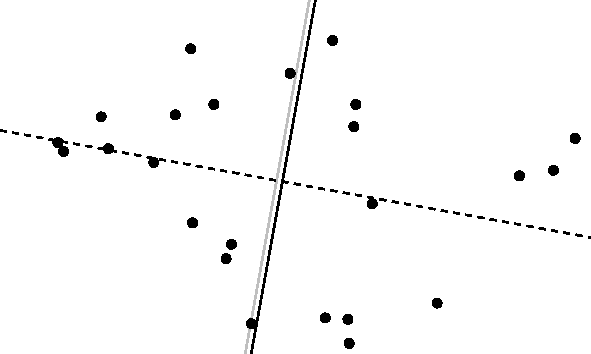
\includegraphics[width=0.85\linewidth]{RIB/RIB_diagram}
          \caption{
            Example of an inertial bisection.
            Vertices are shown as black points, the bisectors of the largest eigen-pair is shown by the black solid, and the bisector of the smallest eigen-pair is shown by the black dashed line.
            The ``shifted'' bisector used in the partitioning is shown in grey.
            While the communication between vertices is not drawn, it is clear that the length (proportional to cut size) of the smallest eigen-pair bisector is larger than that of the largest eigen-pair bisector.
            \label{fig:Spatial Decomposition:RIB Diagram}
          }
        \end{figure}
      }
      %%%%%%%%%%%%%%%%%%%%%%%%%%%%%%%%%%%%%%%%%%%%%%%%%%%%%%%%%%%%%%%%%%%%%%%%%%
      % Recursive Expansion-Based Methods
      %%%%%%%%%%%%%%%%%%%%%%%%%%%%%%%%%%%%%%%%%%%%%%%%%%%%%%%%%%%%%%%%%%%%%%%%%%
      \subsubsection{Recursive Expansion-Based Methods}{\label{sssec:Spatial Decomposition:Recursive Expansion-Based Methods}
        The \ac{REB} methods comprise the last class of partitioning methods examined in this work.
        These methods begin a bisection step by selecting a vertex as the starting point of a subdomain.
        This subdomain is then expanded until it is approximately half the size of the graph \cite{Farhat1988,Nasra1991,Elsner1997,Fitzgerald2017}.
        In this work, the method outlined by \citet{Fitzgerald2017} was slightly modified and generalized to weighted graphs.
        For the remainder of this work, the acronym \emph{\ac{REB}} will be used to denote this specific expansion-based method rather than the entire class of methods.

        This \ac{REB} method considers both the geometry and connectivity of the graph.
        The method begins by choosing a starting vertex for the subdomain and then expands based on a set of prioritized rules.
        At each expansion step, the next vertex is chosen so that it is geometrically close to the vertices within the subdomain and to minimize edges between the subdomain and the remaining graph.
        However, this method makes the assumptions that the mesh is structured, and that every mesh element is the same shape and size.
        For the application in MPACT, this is always true.

        This \ac{REB} method uses the concept of a \emph{\ac{SOI}} around a vertex.
        The \ac{SOI} includes directly neighboring vertices and vertices that neighbor more than one of the direct neighbors or that would if the direct neighbor were present in each structured position around the primary vertex.
        This is shown for 2-D rectangular structured mesh in \cref{fig:Spatial Decomposition:Sphere of Influence}.
        For implementation simplicity, the sphere of influence is calculated using distance rather than connectivity.

        The starting vertex in this \ac{REB} method is chosen using a set of prioritized rules:
        \begin{enumerate}
            \item{must be on graph boundary, i.e. at least one direct neighbor is not present,}
            \item{must have the lowest summed weight of edges, and}
            \item{must be located furthest from weighted centroid (given by \cref{eq:Spatial Decomposition:Mean Coordinates}).}
        \end{enumerate}
        Vertices within the expanding subdomain are considered internal vertices, and the remaining vertices are considered to be external vertices.
        During expansion, the next vertex is determined using a set of prioritized rules:
        \begin{enumerate}
            \item{must be neighboring at least one internal vertex,}
            \item{must have the highest summed weight of edges with internal vertices,}
            \item{must have the lowest summed weight of edges with external vertices,}
            \item{must have the largest number of internal SOI vertices,}
            \item{must have the largest number of external SOI vertices, and}
            \item{must have the smallest distance from reference vertex.}
        \end{enumerate}
        The reference vertex is in the expanding subdomain, which begins as the first vertex but changes during expansion; the reference vertex is the most recently added vertex with less external communication than the previously added vertex.
        An example of the expansion order is shown in \cref{fig:Spatial Decomposition:REB Expansion Order}.

        \begin{algorithm}
          \centering
          \caption{The chosen Recursive Expansion Bisection (REB) algorithm.}
          \label{alg:Recursive Expansion Bisection}
          \begin{algorithmic}[1]
            \Procedure{REB}{$G(V,E)$}
              \State{Compute weighted centroid of the graph}
              \State{Choose a starting vertex for the expanding domain: See rules in \cref{sssec:Spatial Decomposition:Recursive Expansion-Based Methods}}
              \State{Expand the domain from the starting vertex. Let $V_s$ be the list of vertices in order of the expansion: See rules in \cref{sssec:Spatial Decomposition:Recursive Expansion-Based Methods}}
              \State{Cut graph into $G_1(V_1,E_1), G_2(V_2,E_2)$: \Cref{alg:Graph Cutting}}
              \State{REB($G_1(V_1,E_1)$)}
              \State{REB($G_2(V_2,E_2)$)}
            \EndProcedure
          \end{algorithmic}
        \end{algorithm}

        \begin{figure}
          \centering
          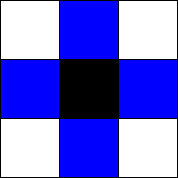
\includegraphics[width=0.45\linewidth]{REB/SoI_Rectangular}
          \caption{
              ``Sphere of influence'' example for 2-D rectangular structured grid.
              The primary vertex is shown in black, direct neighbors are blue, and additional vertices in the sphere are white \cite{Fitzgerald2017}.
              \label{fig:Spatial Decomposition:Sphere of Influence}
          }
        \end{figure}

        \begin{figure}
          \centering
          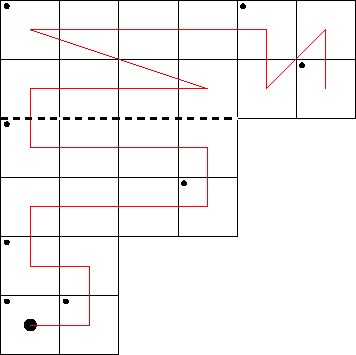
\includegraphics[width=0.65\linewidth]{REB/Expansion}
          \caption{
              An example of the \ac{REB} method expansion on a small graph.
              The black lines show the square mesh cells.
              The expansion begins at the large black point in the center of a cell, and the red line from this shows the expansion's order.
              Each small black dot in the upper left of a cell indicates the reference vertices during expansion.
              The thick black dashed line shows the bisecting cut.
              \label{fig:Spatial Decomposition:REB Expansion Order}
          }
        \end{figure}

      }
    }
  }
  %%%%%%%%%%%%%%%%%%%%%%%%%%%%%%%%%%%%%%%%%%%%%%%%%%%%%%%%%%%%%%%%%%%%%%%%%%%%%%
  % Applications for MPACT
  %%%%%%%%%%%%%%%%%%%%%%%%%%%%%%%%%%%%%%%%%%%%%%%%%%%%%%%%%%%%%%%%%%%%%%%%%%%%%%
  \section{Applications for MPACT}{\label{sec:Spatial Decomposition:Applications for MPACT}
    As described in \cref{sec:Spatial Decomposition:Spatial Decomposition in MPACT}, MPACT's spatial decomposition is performed on the ray-tracing module mesh.
    However, there are a couple of restrictions on spatial subdomains in MPACT.
    Each spatial subdomain must be contiguous, and cannot wrap around other spatial subdomains.
    To account for these restrictions, adaptations are made to the graph partitioning process.

    Due to restrictions in MPACT, at each recursive step, each subdomain in a bisection is made contiguous.
    If a partitioning method results in a noncontiguous subdomain, then each noncontiguous group of modules will be moved into the other subdomain except for the largest group.
    This fix is done at the expense of load-balance, but is necessary for these methods to be robust in MPACT.
    To ensure that no subdomain wraps around another, a fix is applied after the graph partitioning process.
    If a subdomain wraps around another, then the concave subdomain will be given the modules it wraps around.

    A group of ray-tracing modules in MPACT can be abstracted into a graph.
    Each vertex will have weight corresponding to the number of cells contained in the module.
    Edges can be drawn between directly neighboring ray-tracing modules.
    This represents communication in MPACT's \ac{MOC} solver.
    Transport source iterations converge slowly, so MPACT relies on the \ac{CMFD} \cite{Smith1983} acceleration method.
    \ac{CMFD} acceleration is performed by constructing a sparse linear system based on the finite differenced diffusion operator and then solving for the largest eigenpair of that linear system.
    In MPACT, solving the linear system is handled by a third-party library, PETSc \cite{Petsc}.

    For 2-D simulations, the application of graph partitioning methods is clear: abstract the 2-D mesh into a graph for partitioning.
    However, for 3-D, there are additional concerns.
    MPACT's primary 3-D transport method is the 2D-1D method, in which the \ac{MOC} is used in the radial directions, and a lower-order solver couples axial planes \cite{Collins2016}.
    For 2D-1D simulations, MPACT currently restricts spatial domains to be aligned in both the radial and axial directions; this is due to implementation, and is not a general requirement of the methods.

    To comply with MPACT's restrictions on 3-D spatial domains, the current approach is to axially average module weights (numbers of cells), perform a 2-D graph partitioning on a single plane, and apply the resulting partitioning to all axial planes.
    This approach will restrict the number of spatial domains to be an integer multiple of the number of planes.
    This axially and radially aligned scheme is expected to work well in many cases since reactor cores do not typically vary significantly in the axial direction.
    However, for some designs, this may not be true, and planes near the top or bottom of the core have significantly fewer cells; in these cases, high load imbalance is to be expected.

    It is possible to change MPACT's implementation to lift these alignment restrictions.
    If spatial domains were aligned in only the radial direction, there may be some benefit to load-balance.
    In this scheme, each axial plane can be assigned an appropriate number of processes, and a separate 2-D decomposition can be performed for each plane.
    This also lifts restrictions on the number of domains; the number of domains must only be greater than or equal to the number of planes.

    If all alignment restrictions were lifted on MPACT's spatial domains, then a direct partitioning of the 3-D core can be performed by abstracting the entire core to a graph.
    This scheme provides the most freedom and would be expected to give the most balanced decompositions.
    In MPACT's 2D-1D solver, the amount of data communicated radially is significantly larger than that communicated axially, so it may be advantageous to assign the edges connecting the neighboring modules in the axial direction lower weights than those in radial directions.
    By doing so, the overall communication would be expected to be decreased.

    \begin{figure}
      \centering
      \begin{subfigure}[t]{0.3\textwidth}
        \centering
        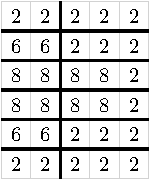
\includegraphics[width=0.9\textwidth]{alignmentComparison/pac_axial}
        \caption{}
      \end{subfigure}%
      ~
      \begin{subfigure}[t]{0.3\textwidth}
        \centering
        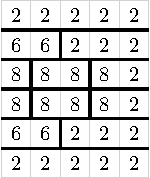
\includegraphics[width=0.9\textwidth]{alignmentComparison/pac_radial}
        \caption{}
      \end{subfigure}%
      ~
      \begin{subfigure}[t]{0.3\textwidth}
        \centering
        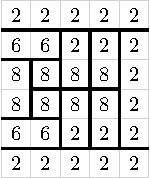
\includegraphics[width=0.9\textwidth]{alignmentComparison/pac_general}
        \caption{}
      \end{subfigure}
      \caption{
        Sample decompositions for (a) axially aligned, (b) radially aligned, and (c) generalized decomposition strategies.
        Rows represent axial planes.
        Numbers are the vertex weights.
        \label{fig:Spatial Decomposition:partitionAlignmentComparison}
      }
    \end{figure}

    \Cref{fig:Spatial Decomposition:partitionAlignmentComparison} shows a comparison of the three hypothetical decomposition schemes, for the purposes of illustration.
    Looking at the \ac{MMR}, as an indicator of load-balance, the strategies have clear differences.
    The \ac{MMR} for the axially aligned, radially aligned, and generalized strategies in this example are $4.00$, $2.67$, and $2.00$, respectively.
    However, it is important to note that the largest domain in each case has the same weight (16), so while the different schemes give different balances, the overall run-times are not expected to be different.
  }
  %%%%%%%%%%%%%%%%%%%%%%%%%%%%%%%%%%%%%%%%%%%%%%%%%%%%%%%%%%%%%%%%%%%%%%%%%%%%%%
  % Results
  %%%%%%%%%%%%%%%%%%%%%%%%%%%%%%%%%%%%%%%%%%%%%%%%%%%%%%%%%%%%%%%%%%%%%%%%%%%%%%
  \section{Results}{\label{sec:Spatial Decomposition:Results}
    %%%%%%%%%%%%%%%%%%%%%%%%%%%%%%%%%%%%%%%%%%%%%%%%%%%%%%%%%%%%%%%%%%%%%%%%%%%%
    % 2-D Results
    %%%%%%%%%%%%%%%%%%%%%%%%%%%%%%%%%%%%%%%%%%%%%%%%%%%%%%%%%%%%%%%%%%%%%%%%%%%%
    \subsection{2-D Results}{\label{ssec:Spatial Decomposition:2-D Results}
      Results were generated for the planar 2-D version of VERA progression problem 5a \cite{VERAProblems}.
      This problem is a quarter core with reflector, barrel, and neutron pad regions surrounding several fuel assemblies, as shown in \cref{fig:Spatial Decomposition:5a-2d}.
      In the model, there are 257 ray-tracing modules in total, which provides the upper bound for the number of domains.
      Each subdomain is assigned to a single processor, with a maximum of 36 processors (subdomains) per computational node.
      Each of the graph decomposition methods was applied to the geometry of this problem, and MPACT was run for each case without applying refinement methods.
      The assembly-based decomposition was run for all possible numbers of subdomains: 1, 4, 16, 73, and 257.
      The possible numbers of subdomains are limited by powers of 4 (8 in 3-D), until subdomains would be located entirely outside the core shape.
      It is also possible to decompose into the fuel assemblies or ray-tracing modules, in this case 73 and 257 respectively.
      Example decompositions for 73 subdomains are shown in \cref{fig:Spatial Decomposition:5a-2d example decomp}.

      \begin{figure}
        \centering
        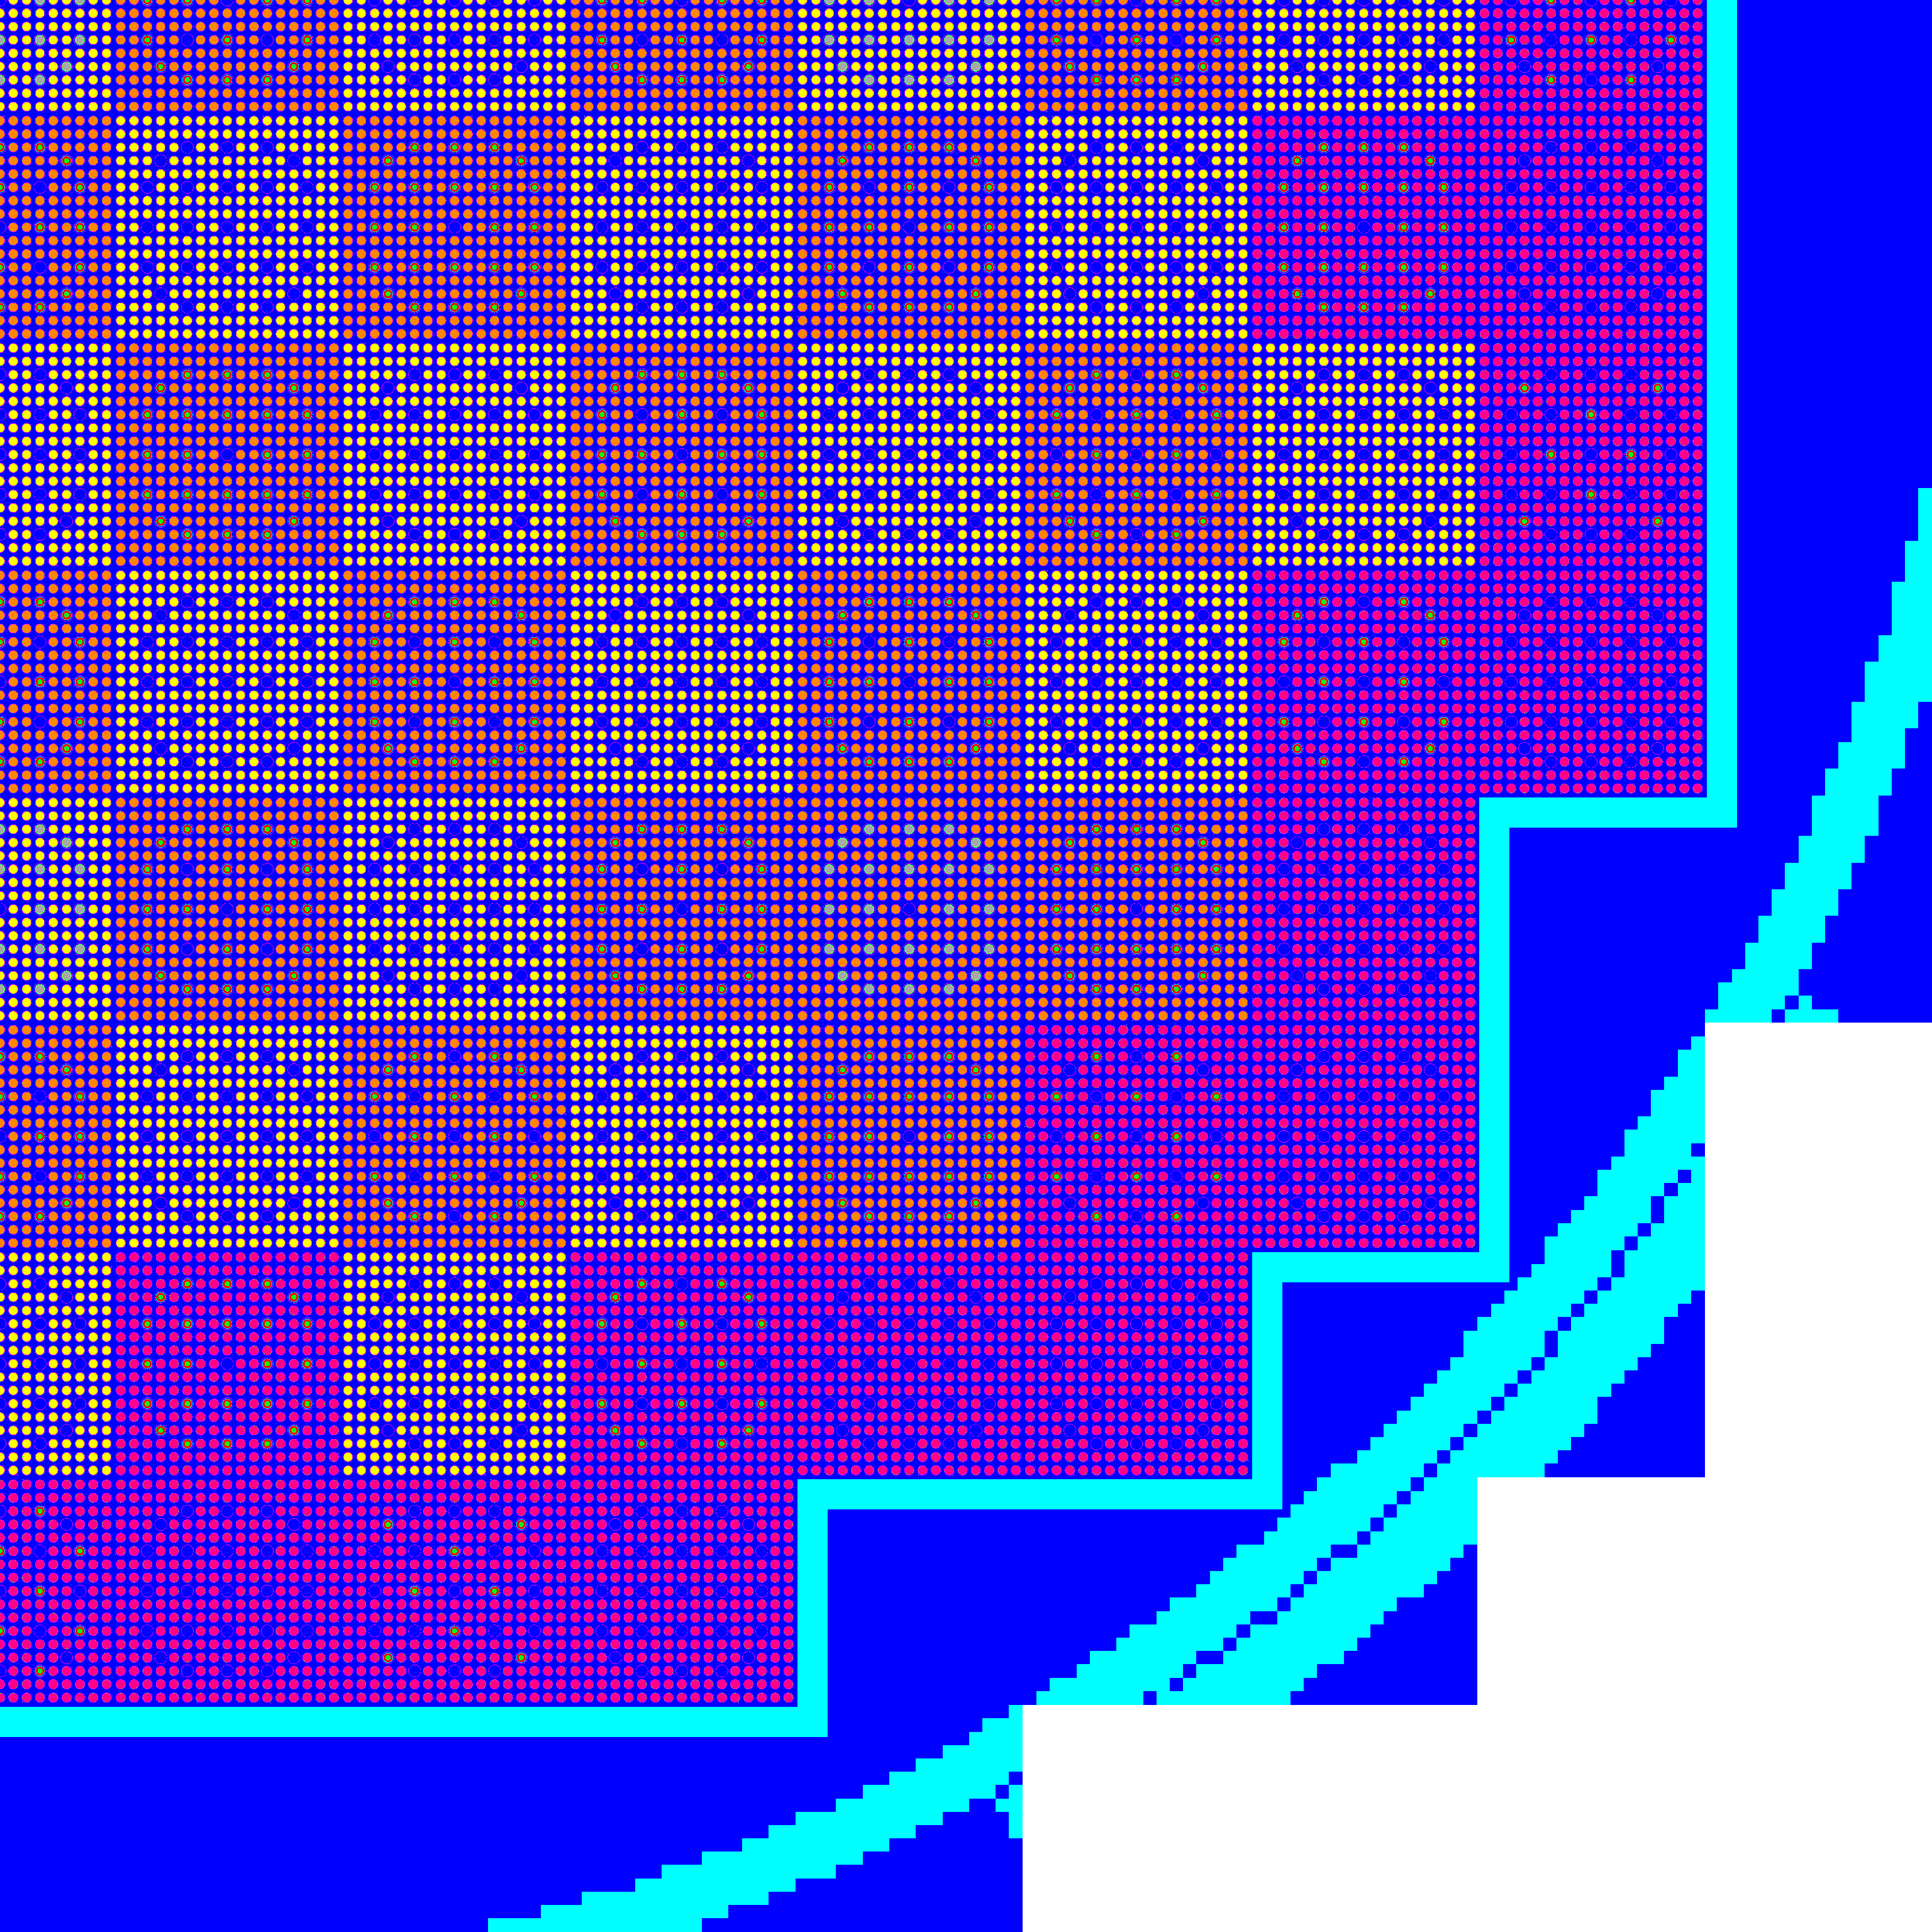
\includegraphics[width=0.35\textwidth]{5a-2d_core}
        \caption{VERA progression problem 5a-2d core configuration. \label{fig:Spatial Decomposition:5a-2d}}
      \end{figure}

      \begin{figure}[H]
        \centering
        \begin{subfigure}[t]{0.45\textwidth}
          \centering
          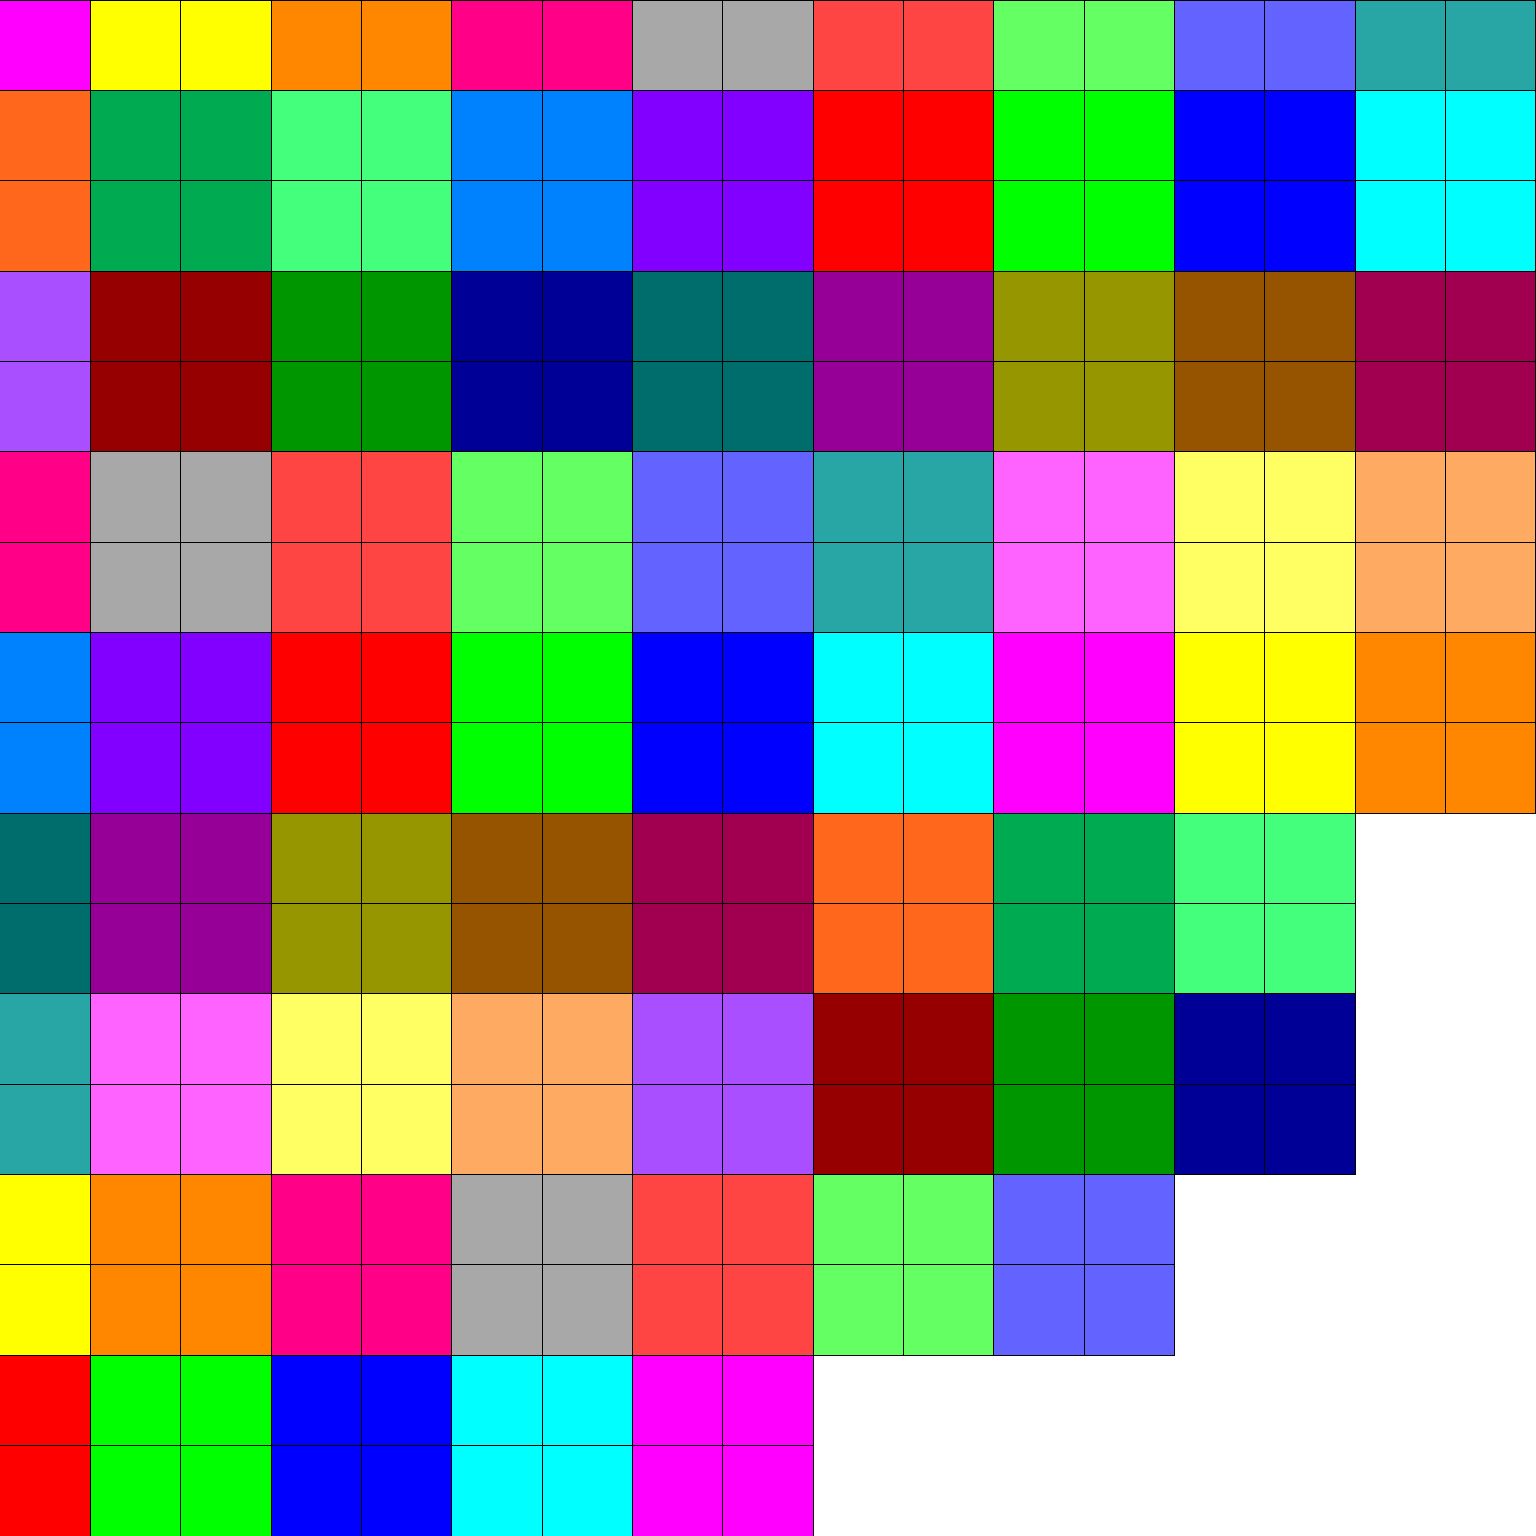
\includegraphics[width=0.9\textwidth]{results/2D/Assembly}
          \caption{Assembly-based decomposition method. \label{fig:Spatial Decomposition:5a-2d 73 Assembly}}
        \end{subfigure}%
        ~
        \begin{subfigure}[t]{0.45\textwidth}
          \centering
          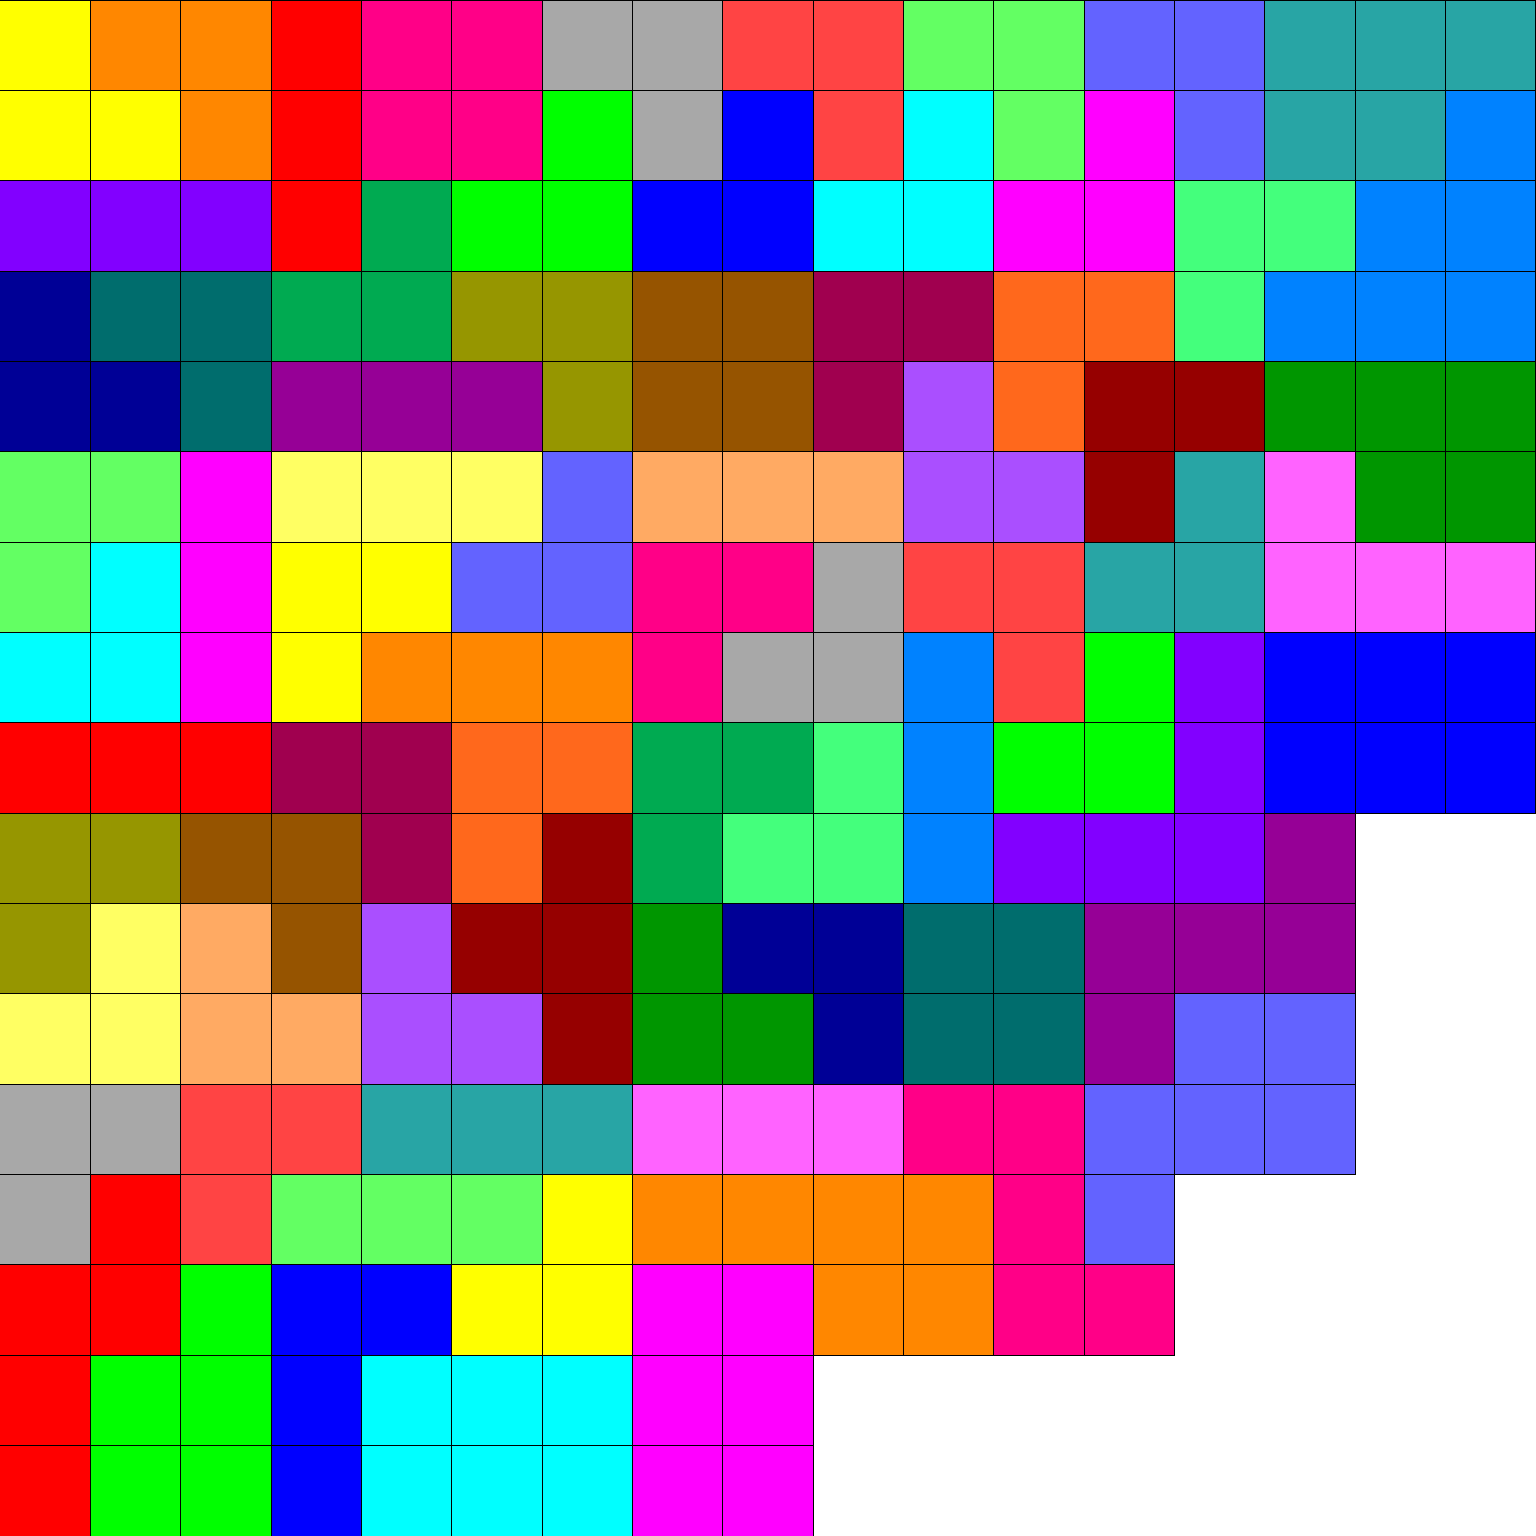
\includegraphics[width=0.9\textwidth]{results/2D/REB_none}
          \caption{\ac{REB} partitioning method. \label{fig:Spatial Decomposition:5a-2d 73 REB None}}
        \end{subfigure}
        \caption{
          Example decompositions for 73 subdomains for VERA progression problem 5a-2d.
          Each color represents a different subdomain.
          \label{fig:Spatial Decomposition:5a-2d example decomp}
        }
      \end{figure}

      %%%%%%%%%%%%%%%%%%%%%%%%%%%%%%%%%%%%%%%%%%%%%%%%%%%%%%%%%%%%%%%%%%%%%%%%%%
      % Load-Balance
      %%%%%%%%%%%%%%%%%%%%%%%%%%%%%%%%%%%%%%%%%%%%%%%%%%%%%%%%%%%%%%%%%%%%%%%%%%
      \subsubsection{Load-Balance}{\label{sssec:Spatial Decomposition:Load-Balance}
        In MPACT, each spatial subdomain is simulated concurrently.
        After each iteration, parallel boundary conditions are communicated and updated in parallel.
        The time for solve routines is measured for each subdomain, as is the \ac{MOC} communication time.
        However, the communication time includes time spent waiting for other subdomains to finish computation; that is, blocking communication.

        This parallel iteration scheme means that the wall-time of each iteration is controlled by the subdomain with the longest run-time; this is expected to be the subdomain with the largest number of cells.
        However, the wall-time is not the only important consideration; it is important to consider how well the computational resources are used.
        A measure for how well computational resources are used is the parallel efficiency, as defined by
        \begin{equation}
            \label{eq:Spatial Decomposition:Parallel Efficiency}
            E \defined \frac{T_s}{N \cdot T},
        \end{equation}
        where $T_s$ is the time in serial, and $T$ is the time in parallel with $N$ processes.

        If runtime is highly correlated with the largest number of cells in a subdomain, then this efficiency is expected to be related to the largest \emph{fraction} of cells in a subdomain.
        Specifically, the parallel efficiency is expected to be inversely proportional to the ratio of the largest fraction of cells to the optimal fraction of cells.
        In an ideally balanced decomposition, each subdomain would have $1/N$ cell fraction.
        By comparing the maximum cell fraction to this optimal value, one can estimate how much longer the simulation will take compared to an ideal decomposition, neglecting serial code sections and overhead.

        Higher parallel efficiency indicates better utilization of the available computational resources, and lower runtime.
        The expectation is that higher parallel efficiency can be obtained by having a largest cell fraction closer to the optimal cell fraction.
        As seen in \cref{fig:Spatial Decomposition:Max/Optimal Ratio}, the \ac{REB} method is expected to have slightly better parallel efficiency than the other methods for many cases.
        It is also expected that for a low number of subdomains, the assembly-based decomposition will result in significantly lower parallel efficiency.
        However, for large numbers of subdomains, the assembly-based decomposition is expected to result in comparable parallel efficiency to the graph partitioning methods.

        \begin{figure}
          \centering
          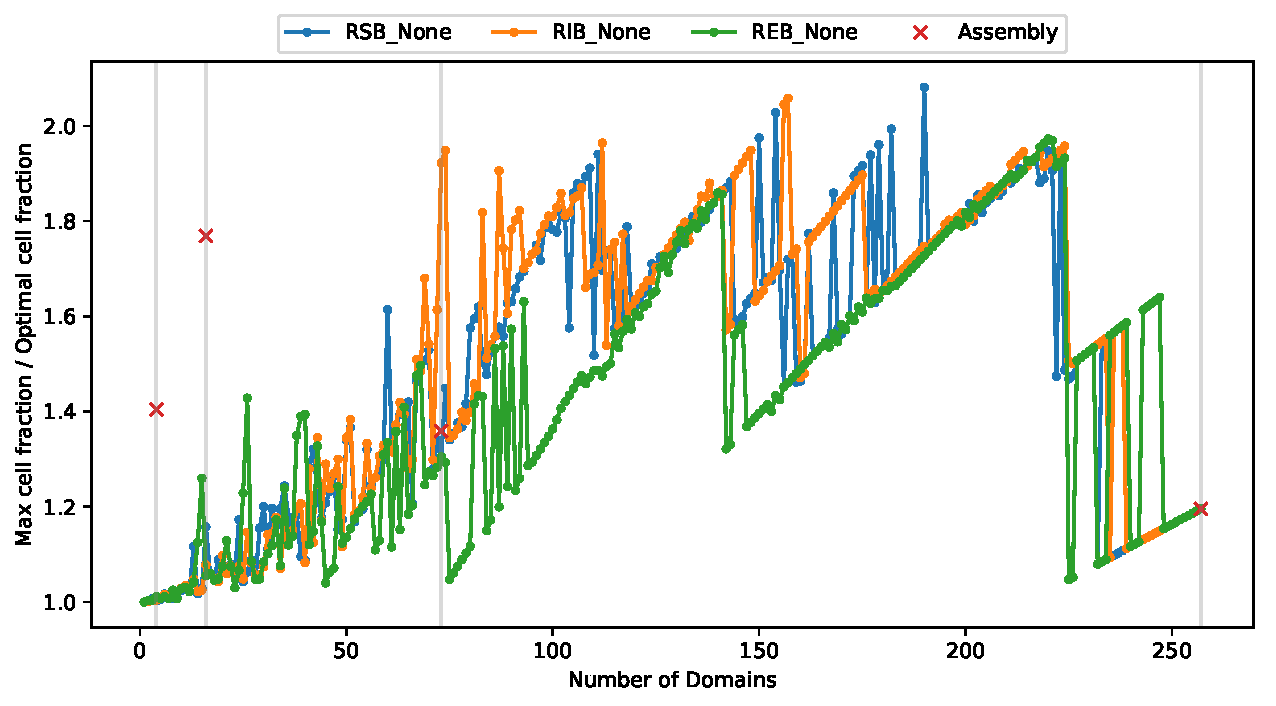
\includegraphics[width=\resultwidth]{results/2D/Size_to_Optimal}
          \caption{Ratio of largest fraction of cells to the optimal fraction of cells as a function of number of subdomains for each partitioning method without refinement.\label{fig:Spatial Decomposition:Max/Optimal Ratio}}
        \end{figure}
      }
      %%%%%%%%%%%%%%%%%%%%%%%%%%%%%%%%%%%%%%%%%%%%%%%%%%%%%%%%%%%%%%%%%%%%%%%%%%
      % Communication
      %%%%%%%%%%%%%%%%%%%%%%%%%%%%%%%%%%%%%%%%%%%%%%%%%%%%%%%%%%%%%%%%%%%%%%%%%%
      \subsubsection{Communication}{\label{sssec:Communication}
        In MPACT, parallel boundary conditions are communicated concurrently.
        However, the measurement of communication time includes any time spent waiting for other subdomains to complete their calculations.
        Generally, the time spent sending receiving parallel boundary conditions is relatively small.
        This time is expected to increase with the weight of edges cut by parallel boundaries.

        \Cref{fig:Spatial Decomposition:2D Communication} shows that the number of edges cut increases as the number of domains increases.
        This indicates that time sending and receiving parallel boundary conditions is expected to increase with the number of subdomains.
        As the number of subdomains increases, the time spent sending and receiving parallel boundary conditions is expected to increase as more data is communicated.
        However, the time difference between the slowest and fastest subdomains decreases, so the overall communication time measurement is expected to decrease.
        Because subdomains in the assembly-based decomposition are rectangular, the number of edges cut is typically lower than in the graph partitioning methods.

        \begin{figure}
          \centering
          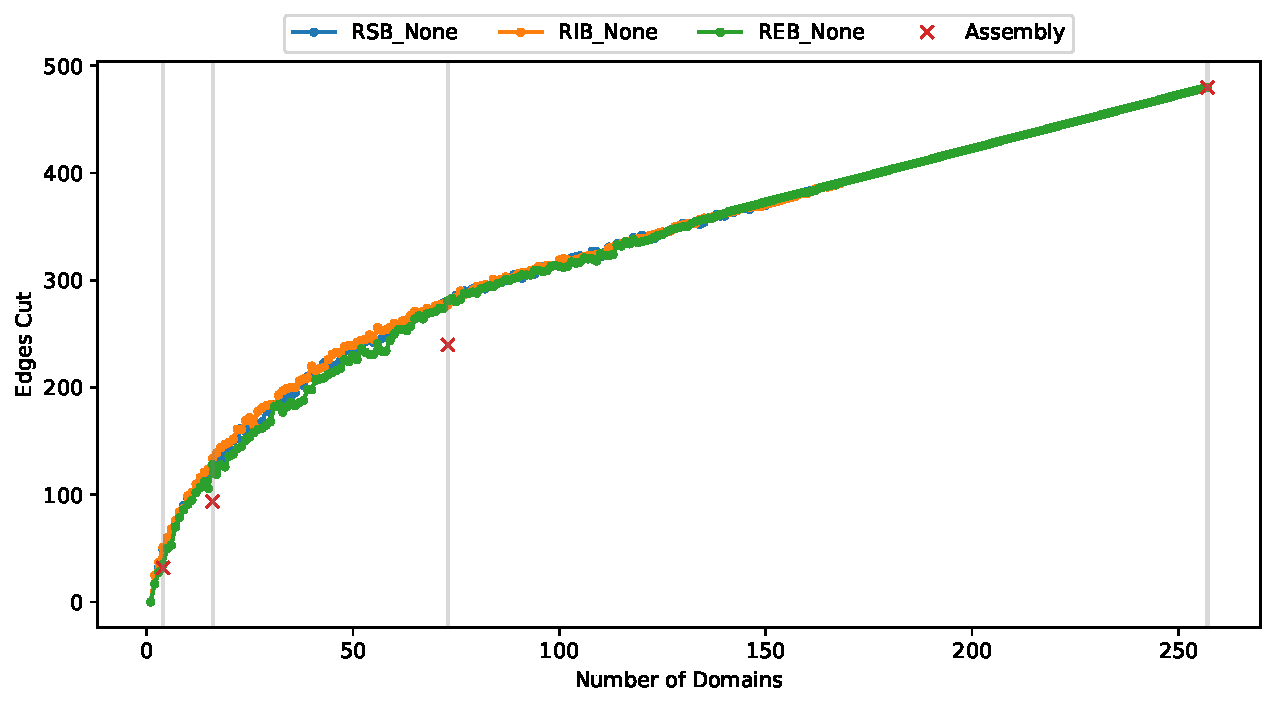
\includegraphics[width=\resultwidth]{results/2D/Edges_Cut}
          \caption{Number of edges cut as a fraction of number of domains for each partitioning method without refinement. \label{fig:Spatial Decomposition:2D Communication}}
        \end{figure}
      }
      %%%%%%%%%%%%%%%%%%%%%%%%%%%%%%%%%%%%%%%%%%%%%%%%%%%%%%%%%%%%%%%%%%%%%%%%%%
      % MPACT Results
      %%%%%%%%%%%%%%%%%%%%%%%%%%%%%%%%%%%%%%%%%%%%%%%%%%%%%%%%%%%%%%%%%%%%%%%%%%
      \subsubsection{MPACT Results}{\label{sssec:MPACT Results}
        As expected, the total and \ac{MOC} run-times are highly correlated with the largest fraction of cells in any subdomain, as shown in \cref{fig:Spatial Decomposition:Runtime Correlation}.
        Both total and \ac{MOC} run-times are very highly correlated with the largest fraction of cells in a subdomain, indicating that this metric can be used to estimate the relative run-times of decompositions.
        The assembly-based decomposition method was not used in this correlation, as there are only a few data points available.

        \begin{figure}
          \centering
          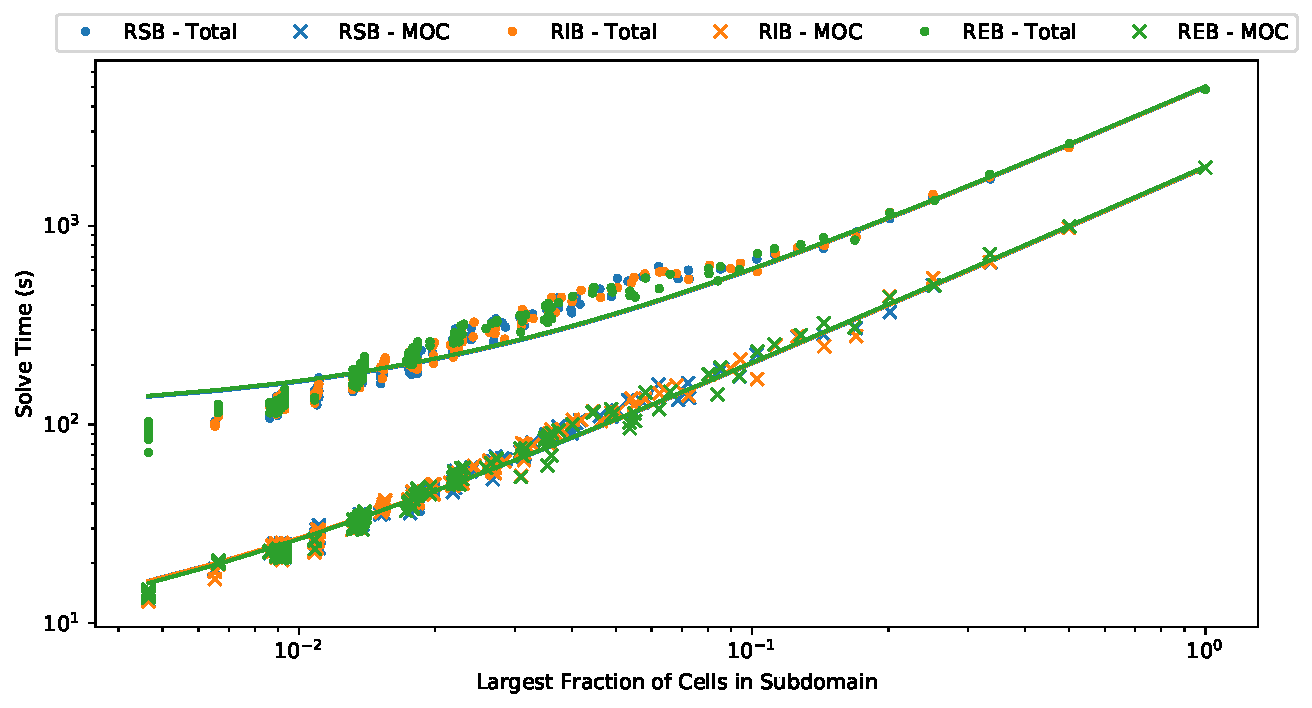
\includegraphics[width=\resultwidth]{results/2D/Run_Time_Fraction_Correlation}
          \caption{Correlation of total and \ac{MOC} run-times to the largest fraction of cells in a subdomain for each partitioning method. \label{fig:Spatial Decomposition:Runtime Correlation}}
        \end{figure}

        Utilization of computational resources is also an important aspect for a high performance simulation code; this can be measured by the parallel efficiency.
        The total parallel efficiency is shown in \cref{fig:Spatial Decomposition:Parallel Efficiency} for each decomposition method.
        As the core becomes more decomposed, the parallel efficiency drops off rapidly, approaching around 20\%.
        Generally, the graph partitioning methods result in similar parallel efficiency, though the \ac{REB} method appears to give very slightly higher efficiency in many cases.
        The assembly-based decomposition method has significantly lower parallel efficiency when there are few subdomains.
        However, for the moderately decomposed problem (73 subdomains) the assembly-based decomposition method results in significantly higher parallel efficiency.
        This was not initially expected, as the largest subdomain has a cell fraction similar to that of the graph partitioning methods.

        \begin{figure}
          \centering
          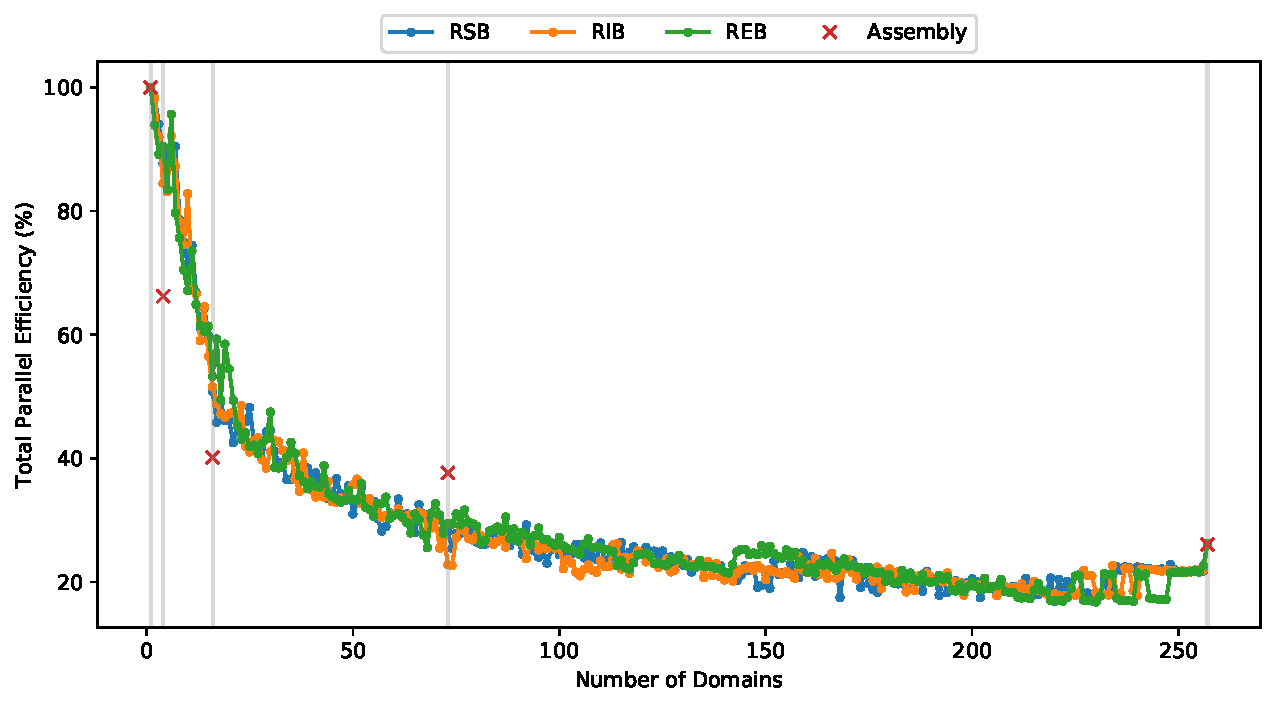
\includegraphics[width=\resultwidth]{results/2D/Total_Parallel_Efficiency}
          \caption{The total parallel efficiency for each partitioning method as a function of the number of domains. \label{fig:Spatial Decomposition:Parallel Efficiency}}
        \end{figure}

        As parallel boundary conditions have a more significant effect on the solution within each subdomain, the convergence rate decreases.
        This occurs as subdomains become smaller (geometrically), or as they become more ``jagged.''
        These jagged parallel boundaries cause re-entrant rays, in which a single ray in the \ac{MOC} will re-enter the subdomain after leaving.
        These re-entrant rays will \emph{not} occur in the assembly-based decomposition, because subdomains are forced to be rectangular.
        This can be observed in \cref{fig:Spatial Decomposition:5a-2d example decomp}.
        The number of \ac{MOC} iterations required for convergence in each case is shown in \cref{fig:Spatial Decomposition:Convergence}.
        There is not a significant increase in the number of outer iterations as the subdomains become smaller, this is consistent with previous results in parallel accelerated transport calculations \cite{Kelley2012,Stimpson2014,Kochunas2014}.
        The increase in number of iterations would be expected to be much more significant in an unaccelerated transport calculation.
        It may be possible to consider spectral information, such as subdomain optical thickness or scattering ratios, during decomposition to allow for a smaller increase in required iterations; however, this will only have an effect at moderately decomposed problems.

        \begin{figure}
          \centering
          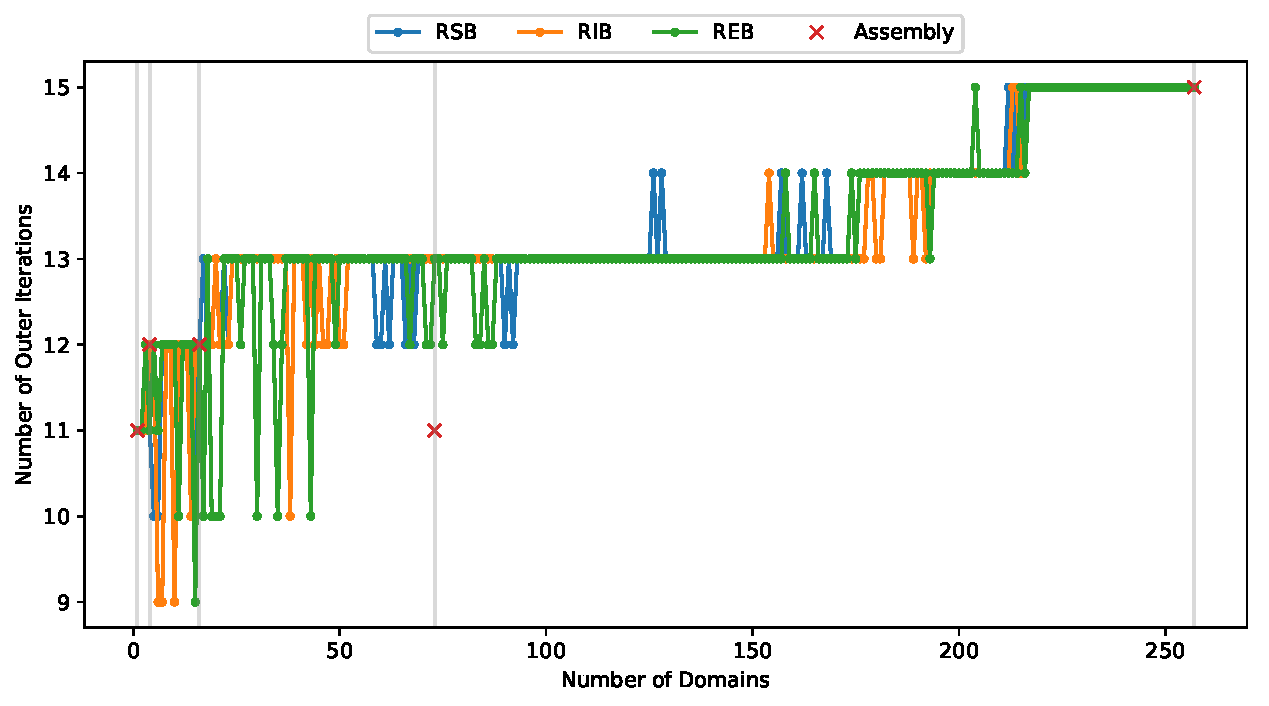
\includegraphics[width=\resultwidth]{results/2D/Convergence_Rates}
          \caption{The number of iterations used by each decomposition method as a function of the number of subdomains. \label{fig:Spatial Decomposition:Convergence}}
        \end{figure}

        By examining the parallel efficiency of \emph{runtime per iteration} these spectral effects are eliminated and the scaling of the solvers in parallel can be determined.
        As shown in \cref{fig:Spatial Decomposition:Scaled Parallel Efficiency}, the total parallel efficiency per iteration decreases as the core becomes more decomposed, limiting toward 25\%.
        However, if only the \ac{MOC} solver time is being examined, the parallel efficiency per iteration decreases at a much slower rate as shown in \cref{fig:Spatial Decomposition:Scaled MOC Parallel Efficiency}.
        This indicates that the \ac{MOC} solver in MPACT is highly efficient in parallel, and that other components of MPACT are the bottleneck in parallel simulations.
        Furthermore, for both total and \ac{MOC} run-times, the graph partitioning methods give comparable parallel efficiencies.
        The assembly-based decomposition method still results in lower efficiency when using few subdomains, but for high numbers of subdomains, it is comparable with the graph partitioning methods.

        \begin{figure}
          \centering
          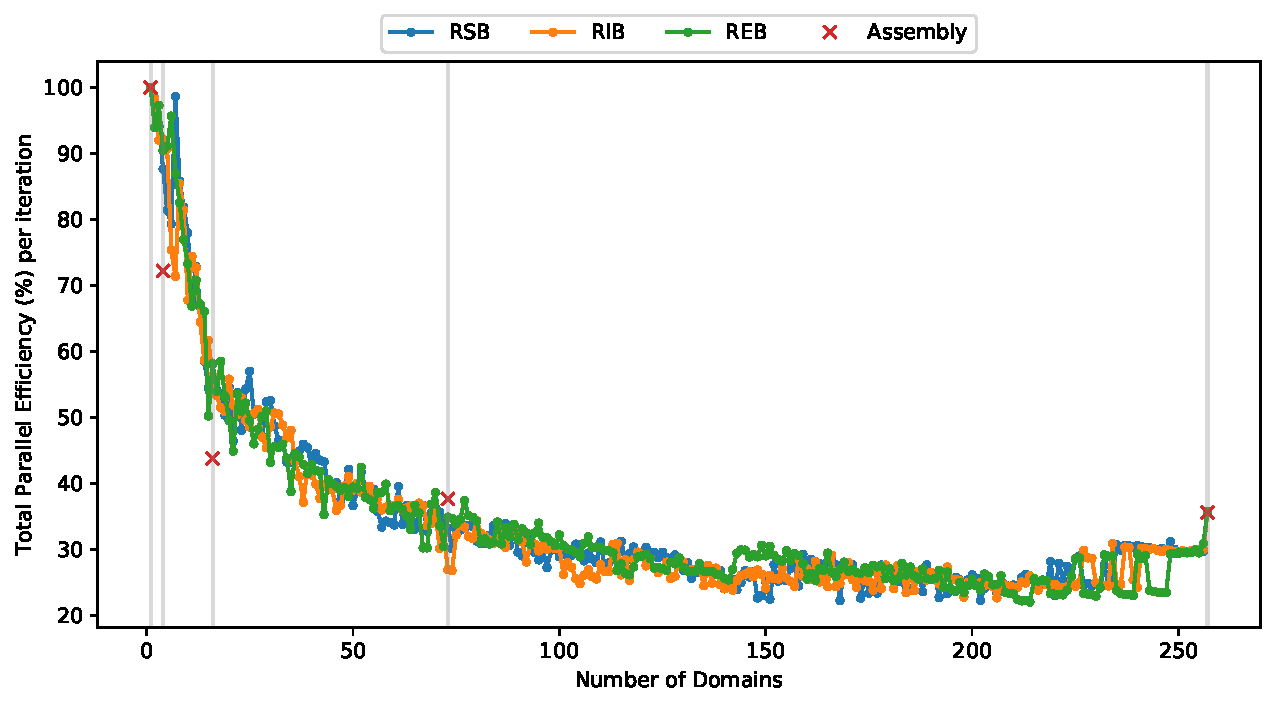
\includegraphics[width=\resultwidth]{results/2D/Scaled_Total_Parallel_Efficiency}
          \caption{The total parallel efficiency per iteration for each partitioning method as a function of the number of domains. \label{fig:Spatial Decomposition:Scaled Parallel Efficiency}}
        \end{figure}

        \begin{figure}
          \centering
          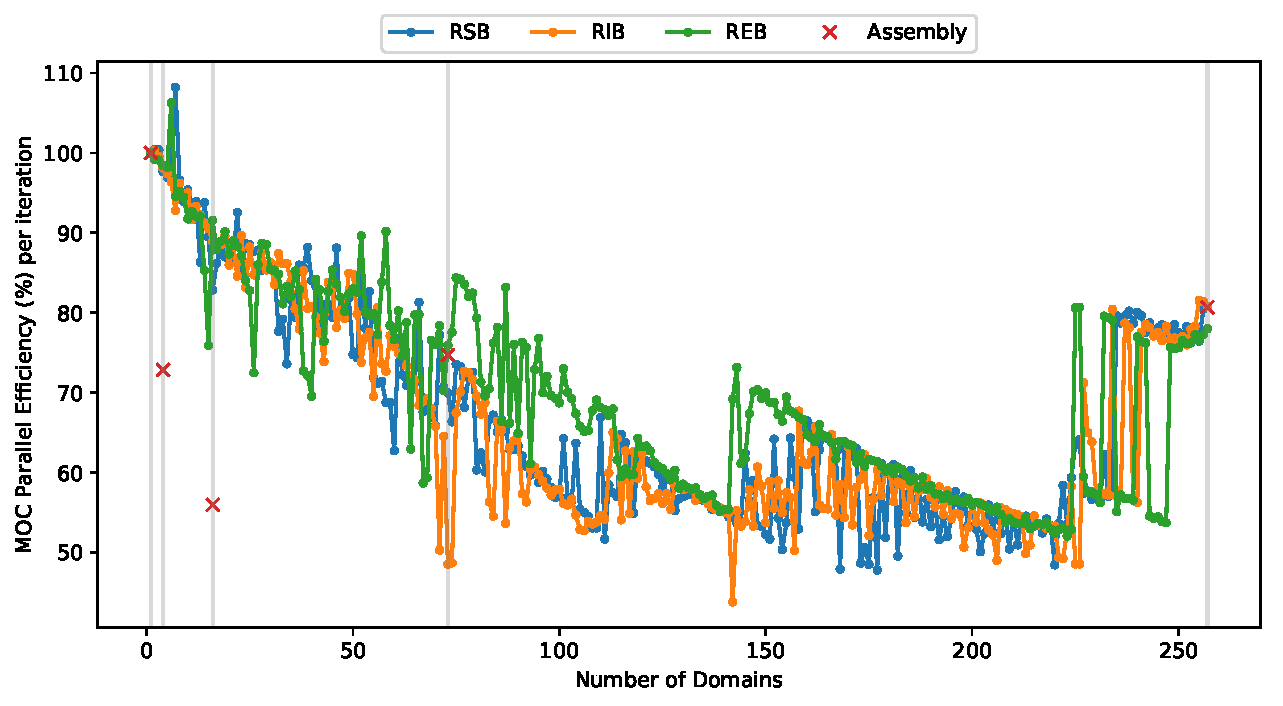
\includegraphics[width=\resultwidth]{results/2D/Scaled_MOC_Parallel_Efficiency}
          \caption{The \ac{MOC} parallel efficiency per iteration for each partitioning method as a function of the number of domains. \label{fig:Spatial Decomposition:Scaled MOC Parallel Efficiency}}
        \end{figure}


        Finally, the ratio of the optimal cell fraction to the maximum cell fraction is expected to be proportional to the parallel efficiency per iteration of the \ac{MOC} solver.
        As shown in \cref{fig:Spatial Decomposition:MOC Parallel Efficiency Correlation}, the parallel efficiency is correlated with the the ratio of optimal-to-maximum cell fractions, though it is not correlated as strongly as the runtime with the maximum cell fraction.
        This indicates that this ratio can be used to estimate the parallel efficiency of the \ac{MOC} solver for a decomposition.
        Even isolating the effect due to increased numbers of iterations, there is a significant spread in parallel efficiency as a function of the optimal to maximum cell fraction ratio; this can be explained by the fact that significantly different numbers of domains (processes) can result in similar fractions.
        This is clearly observed in \cref{fig:Spatial Decomposition:Max/Optimal Ratio}.

        \begin{figure}
          \centering
          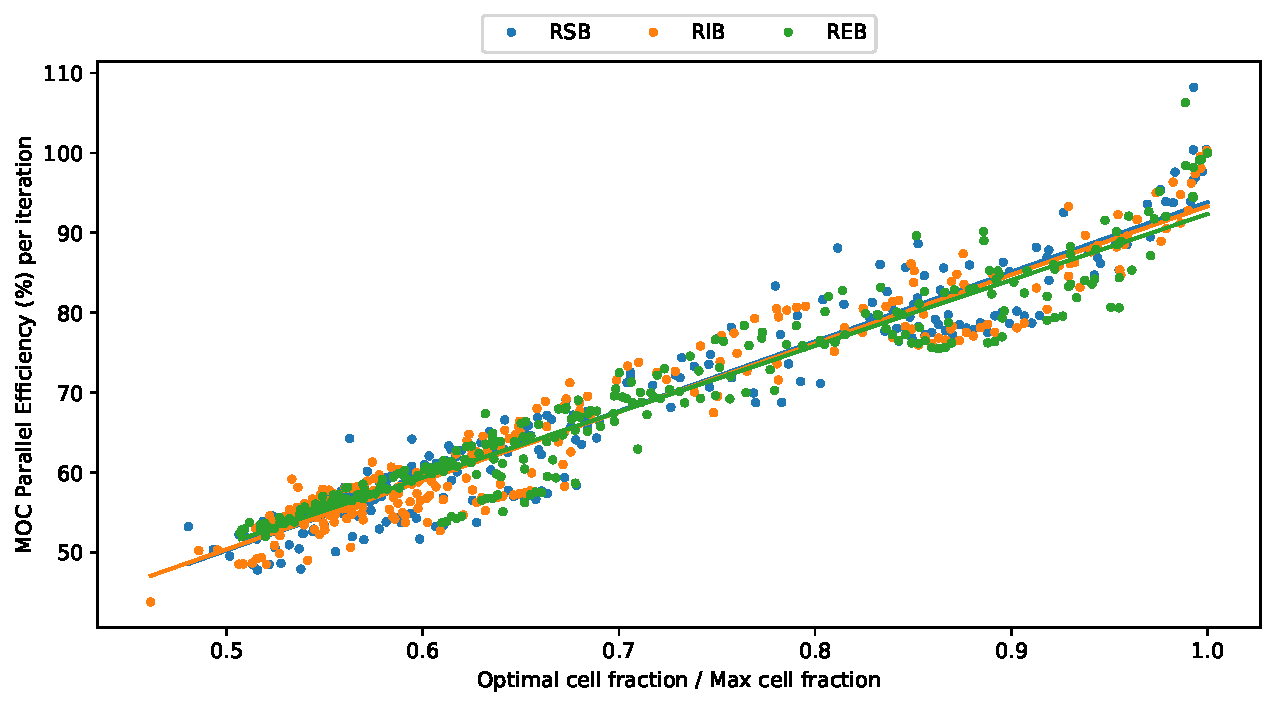
\includegraphics[width=\resultwidth]{results/2D/MOC_Parallel_Efficiency_Correlation}
          \caption{Correlation of the \ac{MOC} parallel efficiency per iteration and the ratio of optimal and maximum cell fractions for each of the partitioning methods. \label{fig:Spatial Decomposition:MOC Parallel Efficiency Correlation}}
        \end{figure}
      }
      %%%%%%%%%%%%%%%%%%%%%%%%%%%%%%%%%%%%%%%%%%%%%%%%%%%%%%%%%%%%%%%%%%%%%%%%%%
      % CMFD Acceleration
      %%%%%%%%%%%%%%%%%%%%%%%%%%%%%%%%%%%%%%%%%%%%%%%%%%%%%%%%%%%%%%%%%%%%%%%%%%
      \subsubsection{CMFD Acceleration}{\label{sssec:CMFD Acceleration}
        In MPACT, the two main solvers contributing to runtime are the \ac{MOC} solver and \ac{CMFD} acceleration, each of which is parallelized using the same computational resources.
        From \cref{fig:Spatial Decomposition:Fractional Runtimes}, the \ac{MOC} and \ac{CMFD} solvers take similar amounts of time in serial; however, as more subdomains are used, the fractional runtime of \ac{CMFD} increases to almost 70\% of the total.
        This indicates that the parallel efficiency is quite low for MPACT's \ac{CMFD} linear system solvers, which heavily leverage PETSc \cite{Petsc} for parallelism.

        \begin{figure}
          \centering
          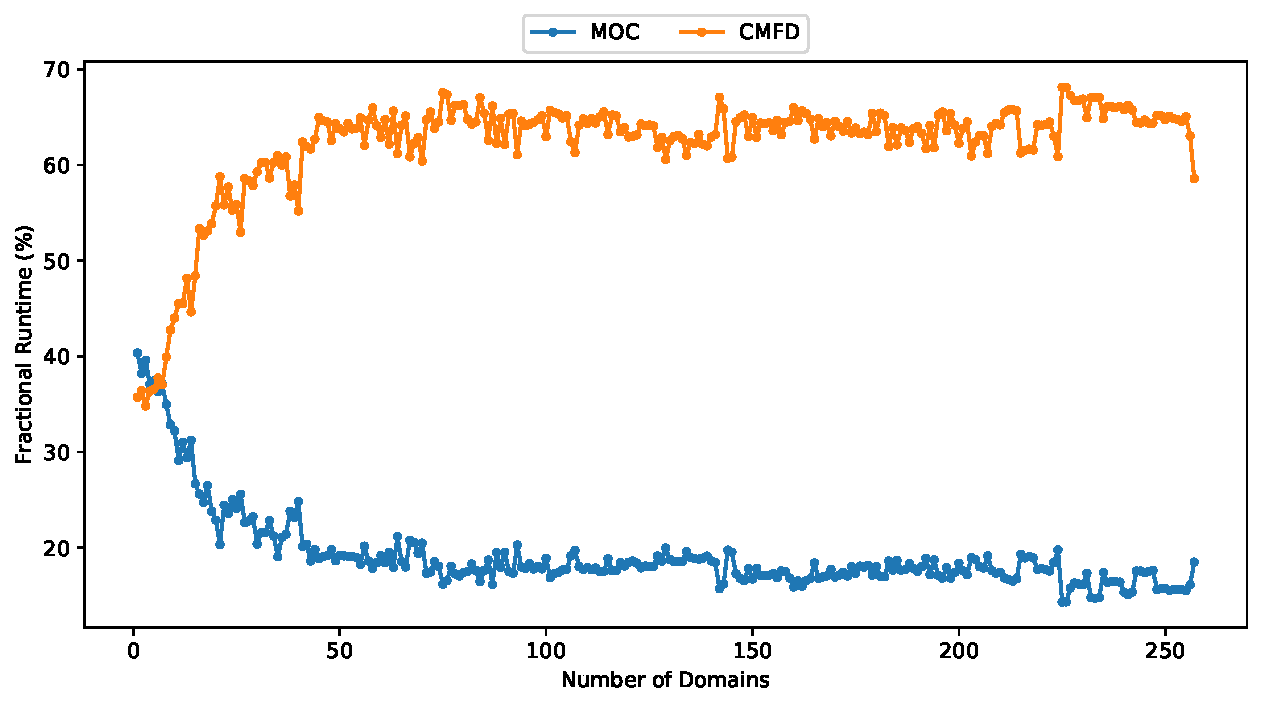
\includegraphics[width=\resultwidth]{results/2D/Fractional_Runtimes}
          \caption{Fractional runtime of the \ac{MOC} solver and \ac{CMFD} acceleration method in MPACT for varying number of domains with the \ac{REB} partitioning method. \label{fig:Spatial Decomposition:Fractional Runtimes}}
        \end{figure}

        Similar as the number of outer transport iterations, as subdomains become smaller, it is expected the \ac{CMFD} linear system will require more iterations for convergence; this is shown for the \ac{REB} partitioning method in \cref{fig:Spatial Decomposition:CMFD Efficiency Summary}.
        However, by considering the parallel efficiency per inner iteration, these convergence effects can be eliminated, and the parallel scaling of the linear system solvers can be examined.
        \Cref{fig:Spatial Decomposition:CMFD Efficiency Summary} shows that the parallel efficiency of the linear system solvers used in MPACT for \ac{CMFD} calculations is quite low, limiting to around 30\%.
        By using a linear system solver that has better parallel scaling \cite{Hao2018}, the overall parallel efficiency of MPACT may be increased.
        However, these results also indicate that the parallel efficiency is, in part, lowered by spectral effects, which will not be eliminated by a more efficient parallel linear solver.

        \begin{figure}
          \centering
          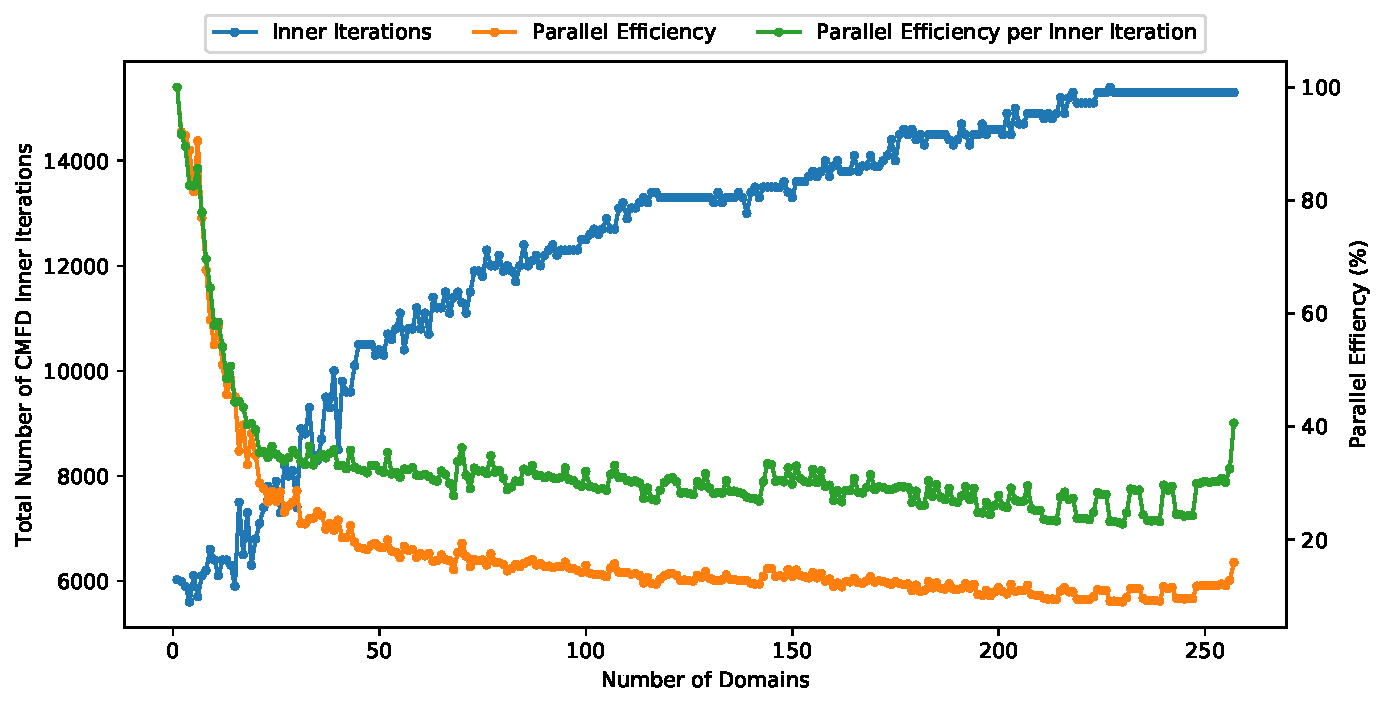
\includegraphics[width=\resultwidth]{results/2D/CMFD_Efficiency_Summary.pdf}
          \caption{The total number of \ac{CMFD} inner iterations, parallel efficiency, and parallel efficiency per inner iteration for varying number of domains with the \ac{REB} partitioning method. \label{fig:Spatial Decomposition:CMFD Efficiency Summary}}
        \end{figure}
      }
    }
    %%%%%%%%%%%%%%%%%%%%%%%%%%%%%%%%%%%%%%%%%%%%%%%%%%%%%%%%%%%%%%%%%%%%%%%%%%%%
    % 3-D Results
    %%%%%%%%%%%%%%%%%%%%%%%%%%%%%%%%%%%%%%%%%%%%%%%%%%%%%%%%%%%%%%%%%%%%%%%%%%%%
    \subsection{3-D Results}{\label{ssec:Spatial Decomposition:3-D Results}
      As shown in \cref{ssec:Spatial Decomposition:2-D Results}, decomposition metrics can be used to estimate the runtime and parallel efficiency without needing to run the simulations.
      There are different approaches to decomposition in 3-D; these are discussed in more detail in \cref{sec:Spatial Decomposition:Applications for MPACT}.
      Decompositions were performed without refinement for three different 3-D decomposition schemes:  \ac{ARA}, \ac{RA}, and \ac{UR}.
      Given fewer restrictions, the resulting decompositions were expected to be more balanced.
      Decompositions were performed on VERA progression problem 5a-0 in 3-D \cite{VERAProblems} with 58 axial planes, but the simulations for this problem were not run.

      The ratio of maximum cell fraction to optimal cell fraction can easily be converted to the maximum cell fraction by dividing by $N$.
      For brevity, only this load balance metric is shown herein.
      The resulting decompositions from the \ac{ARA} approach are very similar to those in the 2-D case.
      Just as in the 2-D case, the maximum-to-optimal cell fraction ratio is lowest for the \ac{REB} method as compared to the other partitioning methods for many cases, as seen in \cref{fig:Spatial Decomposition:3D AR Max. to Optimal Cell Ratio}.
      This indicates that, barring any differences in the number of iterations, the \ac{REB} method is expected to have slightly higher parallel efficiencies.

      \begin{figure}
        \centering
        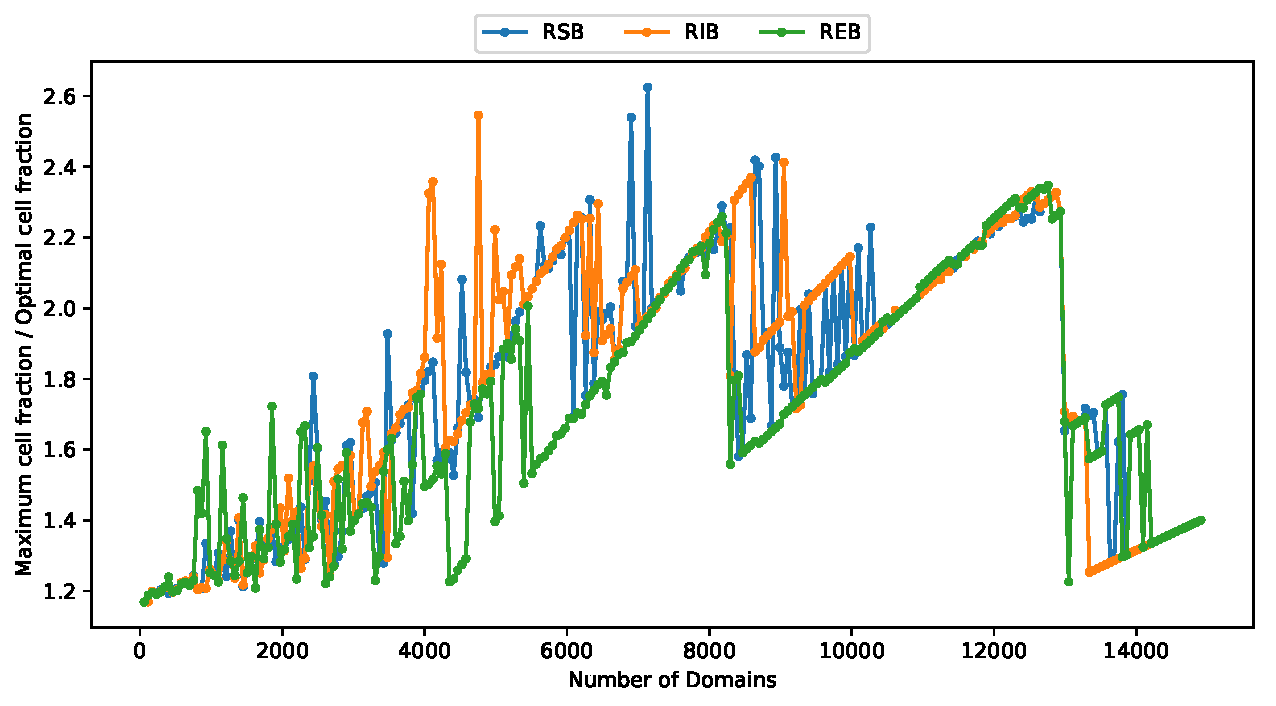
\includegraphics[width=\resultwidth]{results/3D/AxialRadial_Comparison_Ratio}
        \caption{Maximum-to-optimal cell fraction ratio for each partitioning method as a function of number of domains in the \acf{ARA} scheme. \label{fig:Spatial Decomposition:3D AR Max. to Optimal Cell Ratio}}
      \end{figure}

      In the \ac{RA} scheme, a separate decomposition is performed for each axial plane, with an appropriate number of subdomains based on the number of cells in the plane.
      Unlike in the 2-D case, the \ac{REB} method seems to perform significantly worse than the other two methods for low numbers of subdomains.
      For highly decomposed cores, the \ac{REB} method seems to perform slightly better than the other partitioning methods.
      Additionally, by comparing the magnitude of the ratios in \cref{fig:Spatial Decomposition:3D R Max. to Optimal Cell Ratio} and \cref{fig:Spatial Decomposition:3D AR Max. to Optimal Cell Ratio}, it is clear that the \ac{RA} approach typically has less imbalance.

      \begin{figure}
        \centering
        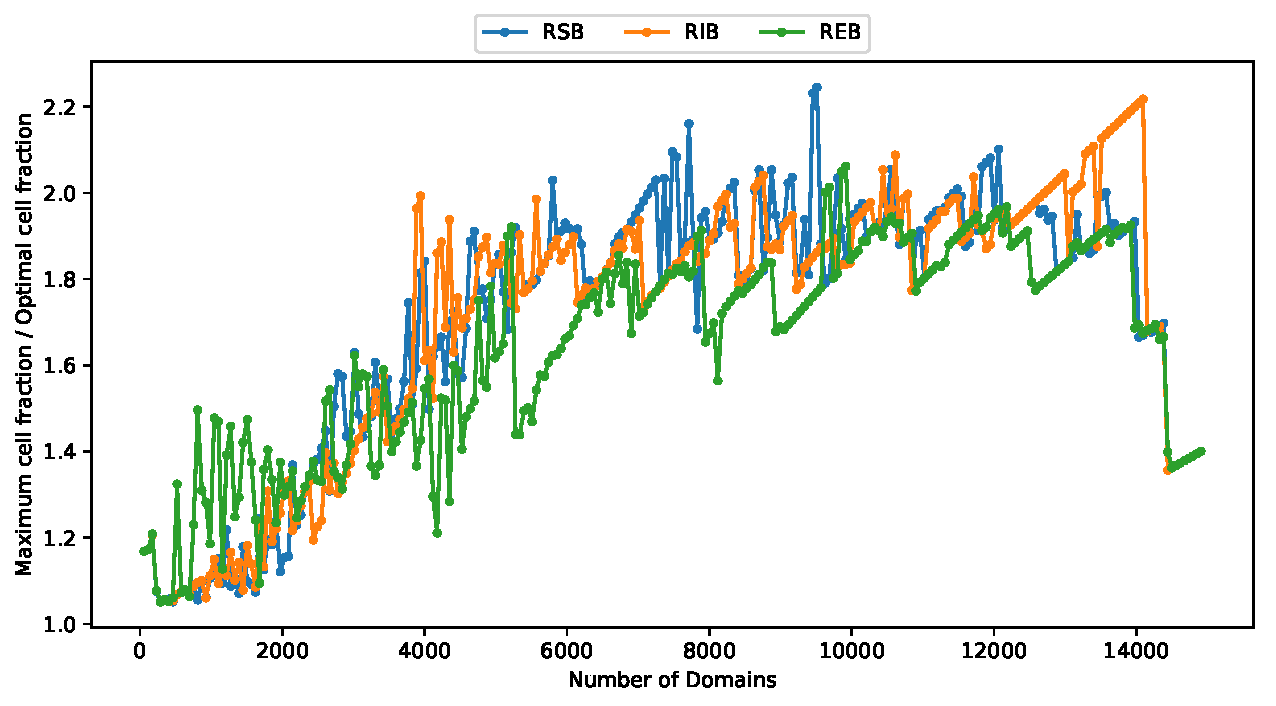
\includegraphics[width=\resultwidth]{results/3D/Radial_Comparison_Ratio}
        \caption{Maximum-to-optimal cell fraction ratio for each partitioning method as a function of number of domains in the \acf{RA} scheme. \label{fig:Spatial Decomposition:3D R Max. to Optimal Cell Ratio}}
      \end{figure}

      Finally, the \ac{UR} approach decomposes the 3-D core by directly abstracting the entire core into a graph.
      The \ac{REB} method is significantly more imbalanced than other methods for lower numbers of subdomains; however, for highly decomposed cores, the \ac{REB} method outperforms the other methods, as shown in \cref{fig:Spatial Decomposition:3D U Max. to Optimal Cell Ratio}.
      Additionally, for highly decomposed problems, both the \ac{RSB} and \ac{RIB} methods seem to have worse balance when using the \ac{UR} scheme compared to the \ac{RA} scheme.

      \begin{figure}
        \centering
        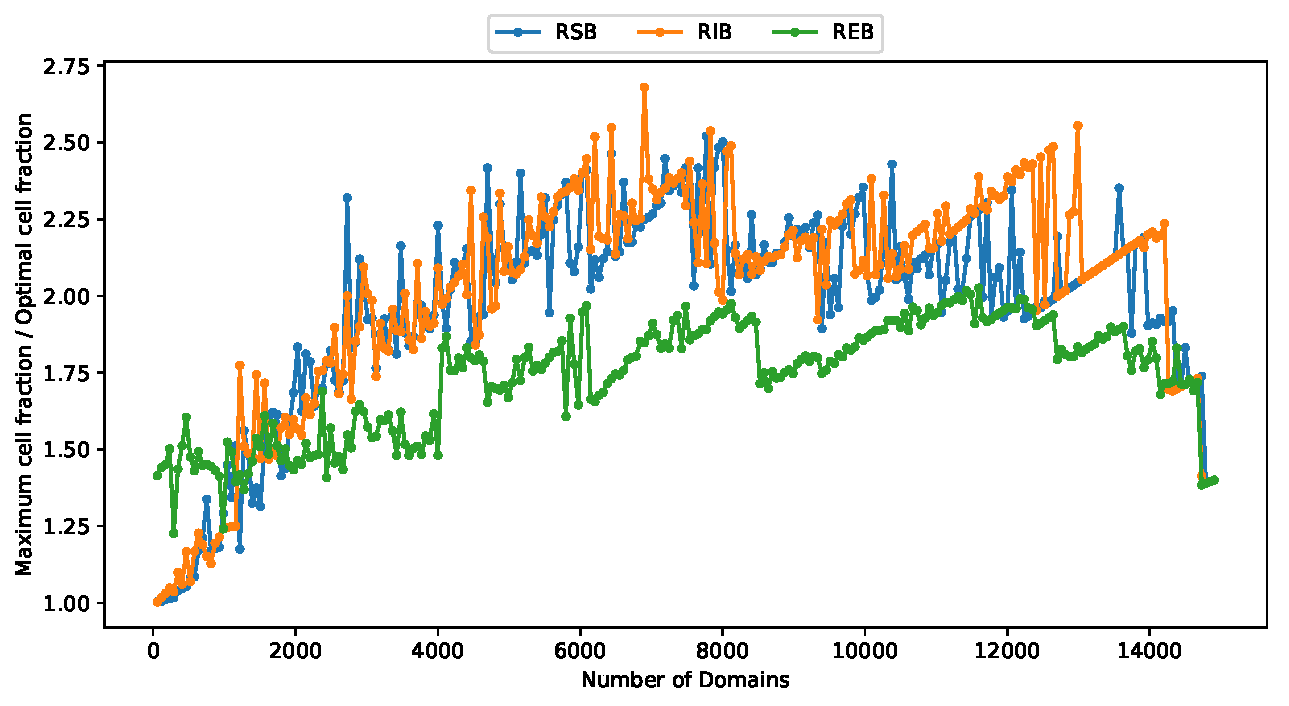
\includegraphics[width=\resultwidth]{results/3D/General_Comparison_Ratio}
        \caption{Maximum-to-optimal cell fraction ratio for each partitioning method as a function of number of domains in the \acf{UR} scheme. \label{fig:Spatial Decomposition:3D U Max. to Optimal Cell Ratio}}
      \end{figure}

      The approach currently used in MPACT is the axially and radially aligned 3-D decomposition scheme.
      If other approaches were to be used, the implementation of parallel communication in the 2D-1D method would need to be reworked.
      To justify these changes, the less restricted approaches would need to offer significant advantages over the current approach.
      \Cref{fig:Spatial Decomposition:RSB 3D Comparison,fig:Spatial Decomposition:RIB 3D Comparison,fig:Spatial Decomposition:REB 3D Comparison} examine the maximum cell fraction of each scheme relative to the current scheme.
      The smaller the relative maximum cell fraction, the lower the expected runtime will be.

      For most applications, reactor cores in MPACT are not highly decomposed with, at maximum, on the order of 30 subdomains per axial plane.
      In this context, modestly decomposed cores are defined as those with fewer than 2,000 subdomains; otherwise, the core is considered highly decomposed.
      For the \ac{RSB} and \ac{RIB} methods, the \ac{RA} approach is expected to give 10\% better performance than the \ac{ARA} approach on average.
      For highly decomposed cases, these partitioning methods are only expected to give an average of 2 -- 3\% better performance.
      On average, the \ac{UR} approach is expected to give \emph{worse} performance by more than 10\% using these partitioning methods.
      However, for the \ac{REB} partitioning method, the \ac{RA} approach is only expected to give 3\% better performance on average.
      Typically, the \ac{UR} approach is still expected to result in worse performance.
      This may be a result of the problem examined in this work which had axial planes that were fairly well balanced.
      By giving the graph partitioning methods more degrees of freedom the heuristic graph partitioning methods perform worse overall.
      Multi-level partitioning methods reduce the degrees of freedom during coarsening and may be more appropriate in these cases.

      \begin{figure}
        \centering
        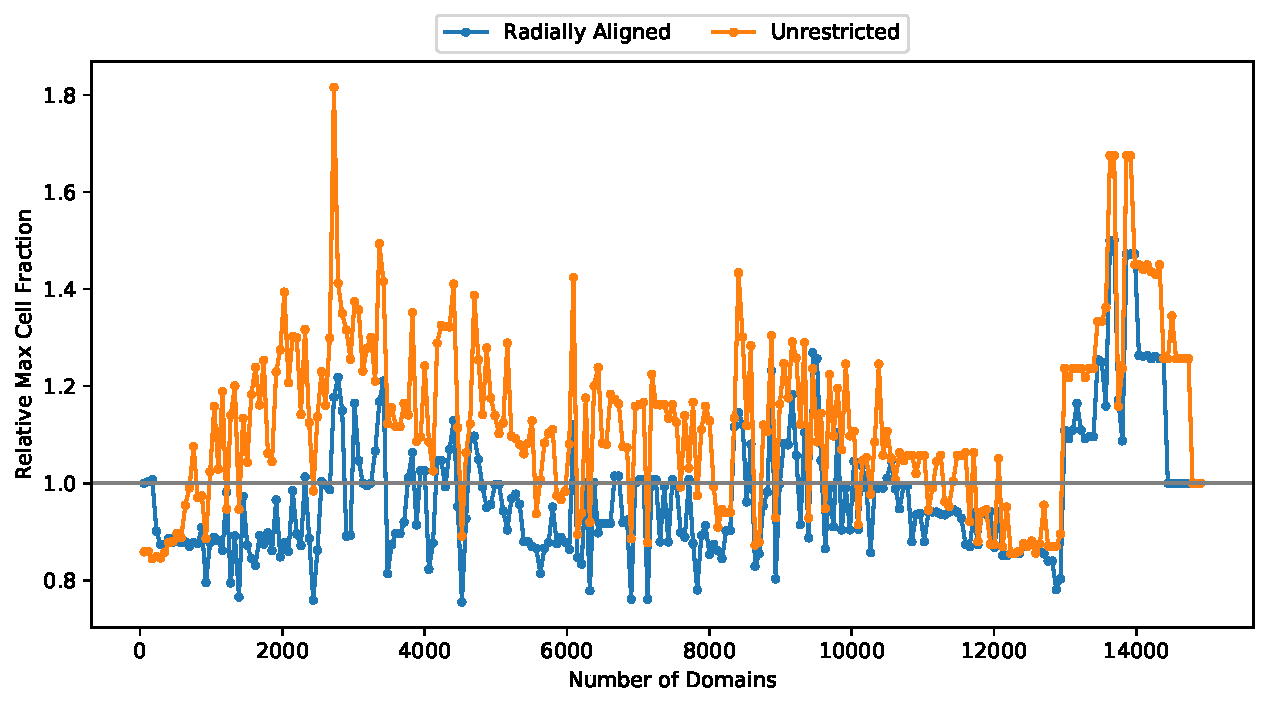
\includegraphics[width=\resultwidth]{results/3D/RSB_Comparison}
        \caption{Maximum cell fraction relative to the \acf{ARA} approach for the \ac{RSB} partitioning method. \label{fig:Spatial Decomposition:RSB 3D Comparison}}
      \end{figure}
      \begin{figure}
        \centering
        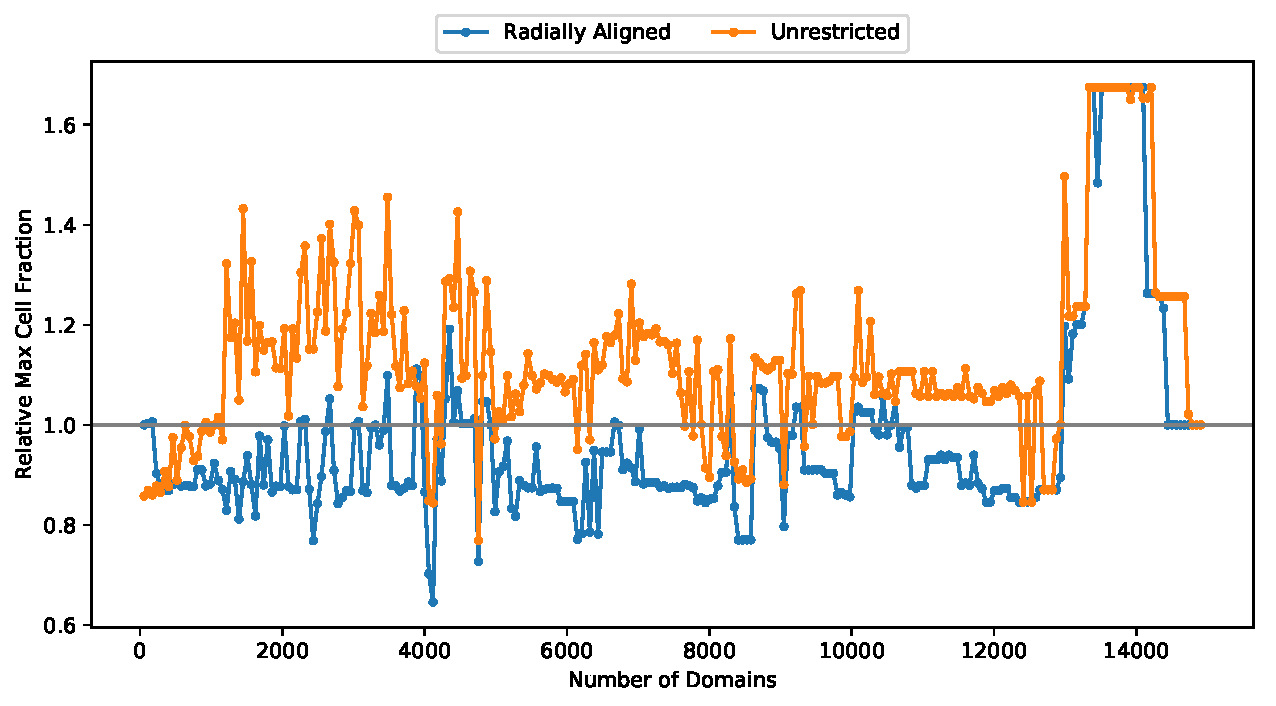
\includegraphics[width=\resultwidth]{results/3D/RIB_Comparison}
        \caption{Maximum cell fraction relative to the \acf{ARA} approach for the \ac{RIB} partitioning method. \label{fig:Spatial Decomposition:RIB 3D Comparison}}
      \end{figure}
      \begin{figure}
        \centering
        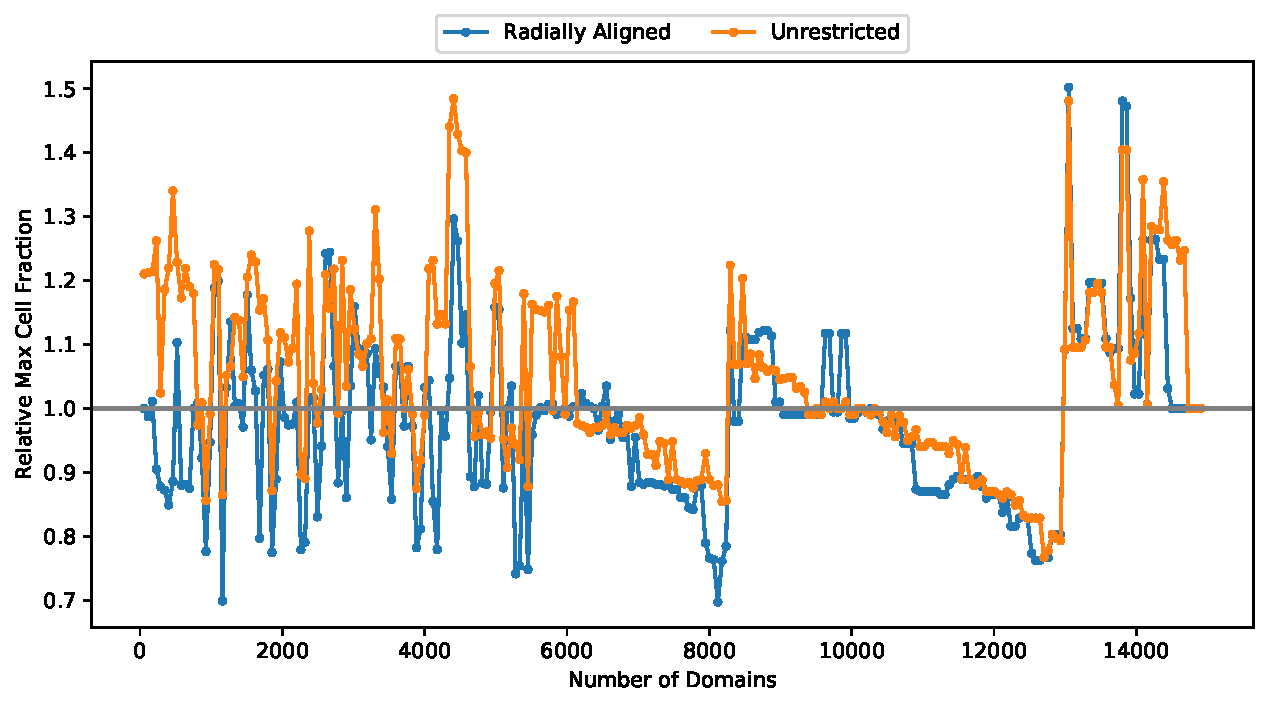
\includegraphics[width=\resultwidth]{results/3D/REB_Comparison}
        \caption{Maximum cell fraction relative to the \acf{ARA} approach for the \ac{REB} partitioning method. \label{fig:Spatial Decomposition:REB 3D Comparison}}
      \end{figure}
    }
  }
  %%%%%%%%%%%%%%%%%%%%%%%%%%%%%%%%%%%%%%%%%%%%%%%%%%%%%%%%%%%%%%%%%%%%%%%%%%%%%%
  % Partition Refinement Methods
  %%%%%%%%%%%%%%%%%%%%%%%%%%%%%%%%%%%%%%%%%%%%%%%%%%%%%%%%%%%%%%%%%%%%%%%%%%%%%%
  \section{Partition Refinement}{\label{sec:Spatial Decomposition:Partition Refinement}
    %%%%%%%%%%%%%%%%%%%%%%%%%%%%%%%%%%%%%%%%%%%%%%%%%%%%%%%%%%%%%%%%%%%%%%%%%%%%
    % Partition Refinement Methods
    %%%%%%%%%%%%%%%%%%%%%%%%%%%%%%%%%%%%%%%%%%%%%%%%%%%%%%%%%%%%%%%%%%%%%%%%%%%%
    \subsection{Partition Refinement Methods}{\label{ssec:Spatial Decomposition:Partition Refinement Methods}
      The Kernighan-Lin algorithm \cite{Kernighan1970} is often described as one of the earliest developed graph partitioning algorithms; however, the algorithm does not actually create a partitioning of the graph, it improves, or refines, the quality by reducing the number of edges cut between existing partitions \cite{Elsner1997}.
      Therefore, in this work, this method and a modified version of it are called \emph{refinement methods}.

      As suggested by Pothen \cite{Pothen1989}, the \ac{RSB} method or other partitioning methods can create a high quality initial partitioning to use in the Kernighan-Lin algorithm.
      Significant improvements have been made to the efficiency of the original Kernighan-Lin algorithm \cite{Fiduccia1982}; however, the graphs of concern in this work are relatively small, and graph decomposition time is negligible when compared to the overall simulation runtime.
      Two partition refinement methods were examined: the Kernighan-Lin algorithm \cite{Kernighan1970} and a modification to the Kernighan-Lin algorithm which takes some geometric information of the graph into account \cite{Fitzgerald2017}.

      The investigated partition refinement algorithms reduce the weight of edges cut between two partitions by swapping vertex pairs between the partitions iteratively.
      The original Kernighan-Lin algorithm operates entirely on the connectivity of the graph, while the modified Spatial Kernighan-Lin algorithm uses both connectivity and geometric information from the graph.

      For each vertex in the graph, $D$ is defined as
      \begin{equation}
          \label{eq:Spatial Decomposition:KL D}
          D_i \equiv E_{E,i} - E_{I,i},
      \end{equation}
      where $E_{E,i}$ is the sum of edge weights from vertex $i$ connecting with vertices outside the partition containing vertex $i$, and $E_{I,i}$ is the sum of edge weights from vertex $i$ connecting with vertices within the partition containing vertex $i$.
      The reduction in communication or ``gain,'' from swapping a pair of vertices $(a,b)$ is defined as
      \begin{equation}
          \label{eq:Spatial Decomposition:KL gain}
          g_{(a,b)} \equiv D_a + D_b - 2c_{a,b}.
      \end{equation}

      The Kernighan-Lin algorithm, given in \cref{alg:Kernighan-Lin}, is a greedy algorithm, in that it will swap a pair $(a,b)$ with maximal $g$ at the current step.
      The idea is that by doing this iteratively, the algorithm will lead to a minimized cut-size; in reality, the algorithm will often get stuck in local minima that do not have a global minimized cut-size.
      Additionally, there may be multiple pairs $(a,b)$ with the same maximal gain value: the algorithm will only consider one of these pairs.

      The Spatial Kernighan-Lin algorithm, given in \cref{alg:Spatial Kernighan-Lin}, is an adaptation of the Kernighan-Lin algorithm which accounts for the multiple pairs with maximal gain.
      This algorithm prioritizes vertex pairs which are geometrically distant from one another.
      The idea behind this modification is that to minimize the edge-cut, the cut should be as straight as possible.
      By prioritizing distant vertex pairs, the bisector is typically ``straightened'' out; this process can be likened to pulling on the ends of a string in order to straighten it.

      \begin{algorithm}
        \centering
        \caption{Kernighan-Lin Algorithm, with input graph $G(V,E)$, and vertex sets $A$ and $B$ within the graph.}
        \label{alg:Kernighan-Lin}
        \begin{algorithmic}[1]
          \Procedure{Kernighan-Lin}{$G(V,E), A, B$}
            \State{$g_m = 1$}
            \While{$g_m > 0$}
              \State{$W_A = \suml[i \in A]w_i$}
              \State{$W_B = \suml[i \in B]w_i$}
              \State{Compute $D \ \forall \ V$ (\Cref{eq:Spatial Decomposition:KL D})}
              \State{Let $a_v, b_v, g_v$ be empty sets}
              \For{$n=1$~to~$N/2$}
                \State{Find unmarked pair $(a,b)$ such that:
                    \begin{enumerate}[leftmargin=2.5cm]
                        \item{$a \in A$ and $b \in B$}
                        \item{$g$ is maximized (\Cref{eq:Spatial Decomposition:KL gain})}
                    \end{enumerate}
                }
                \State{$\widehat{W}_A = W_A + w_b - w_a$}
                \State{$\widehat{W}_B = W_B + w_a - w_b$}
                \If{MAX($W_A$, $W_B$) $\geq$ MAX($\widehat{W}_A, \widehat{W}_B$)}
                  \State{Append $a$ to $a_v$, $b$ to $b_v$, and $g$ to $g_v$}
                  \State{Update $D$ values as if $a,b$ have been swapped}
                  \State{$W_A = \widehat{W}_A$}
                  \State{$W_A = \widehat{W}_B$}
                \Else
                  \State{End search}
                \EndIf
              \EndFor
              \State{Find $k$ maximizing $g_m = \suml[i=1][k]g_v(i)$}
              \If{$g_m > 0$}
                \State{Exchange vertices in $a_v(1:k)$ and $b_v(1:k)$}
              \EndIf
            \EndWhile
          \EndProcedure
        \end{algorithmic}
      \end{algorithm}

      \begin{algorithm}
        \centering
        \caption{Spatial Kernighan-Lin Algorithm, with input graph $G(V,E)$, and vertex sets $A$ and $B$ within the graph.}
        \label{alg:Spatial Kernighan-Lin}
        \begin{algorithmic}[1]
          \Procedure{Spatial Kernighan-Lin}{$G(V,E), A, B$}
            \State{$g_m = 1$}
            \While{$g_m > 0$}
              \State{$W_A = \suml[i \in A]w_i$}
              \State{$W_B = \suml[i \in B]w_i$}
              \State{Compute $D \ \forall \ V$ (\Cref{eq:Spatial Decomposition:KL D})}
              \State{Let $a_v, b_v, g_v$ be empty sets}
              \For{$n=1$~to~$N/2$}
                \State{Allow $(f_a,f_b)$ to be sets from $A,B$ satisfying:
                    \begin{enumerate}
                        \item{$a \in A$, $b \in B$}
                        \item{$g$ is maximized (\Cref{eq:Spatial Decomposition:KL gain})}
                        \item{$a$ and $b$ are on the boundary between $A$ and $B$}
                    \end{enumerate}
                }
                \State{Find pair $(f_a',f_b')$ such that distance is maximized}
                \If{No pair found}
                  \State{Search using standard Kernighan-Lin rules}
                \EndIf
                \State{$\widehat{W}_A = W_A + w_b - w_a$}
                \State{$\widehat{W}_B = W_B + w_a - w_b$}
                \If{MAX($W_A$, $W_B$) $\geq$ MAX($\widehat{W}_A, \widehat{W}_B$)}
                  \State{Append $a$ to $a_v$, $b$ to $b_v$, and $g$ to $g_v$}
                  \State{Update $D$ values as if $a,b$ have been swapped}
                  \State{$W_A = \widehat{W}_A$}
                  \State{$W_A = \widehat{W}_B$}
                \Else
                  \State{End search}
                \EndIf
              \EndFor
              \State{Find $k$ maximizing $g_m = \suml[i=1][k]g_v(i)$}
              \If{$g_m > 0$}
                \State{Exchange vertices in $a_v(1:k)$ and $b_v(1:k)$}
              \EndIf
            \EndWhile
          \EndProcedure
        \end{algorithmic}
      \end{algorithm}
    }
    %%%%%%%%%%%%%%%%%%%%%%%%%%%%%%%%%%%%%%%%%%%%%%%%%%%%%%%%%%%%%%%%%%%%%%%%%%%%
    % Partition Refinement Results
    %%%%%%%%%%%%%%%%%%%%%%%%%%%%%%%%%%%%%%%%%%%%%%%%%%%%%%%%%%%%%%%%%%%%%%%%%%%%
    \subsection{Partition Refinement Results}{\label{ssec:Spatial Decomposition:Partition Refinement Results}
      In \cref{ssec:Spatial Decomposition:Partition Refinement Methods}, refinement methods are introduced as a method for further reducing communication.
      \Cref{fig:Spatial Decomposition:2D RSB Refinement} shows that both refinement methods are able to slightly reduce the number of edges cut compared to the cases without refinement for \ac{RSB}.
      Similar trends are observed for the other partitioning methods.
      While these refinement methods offer a slight reduction in communication, the parallel efficiency due to load imbalance may be negatively affected by applying refinement, as shown in \cref{fig:Spatial Decomposition:RSB Refinement Balance}.
      Communication is not expected to have as significant of an effect as load imbalance, so for the simulations in MPACT, partitioning methods were used without refinement.

      \begin{figure}
        \centering
        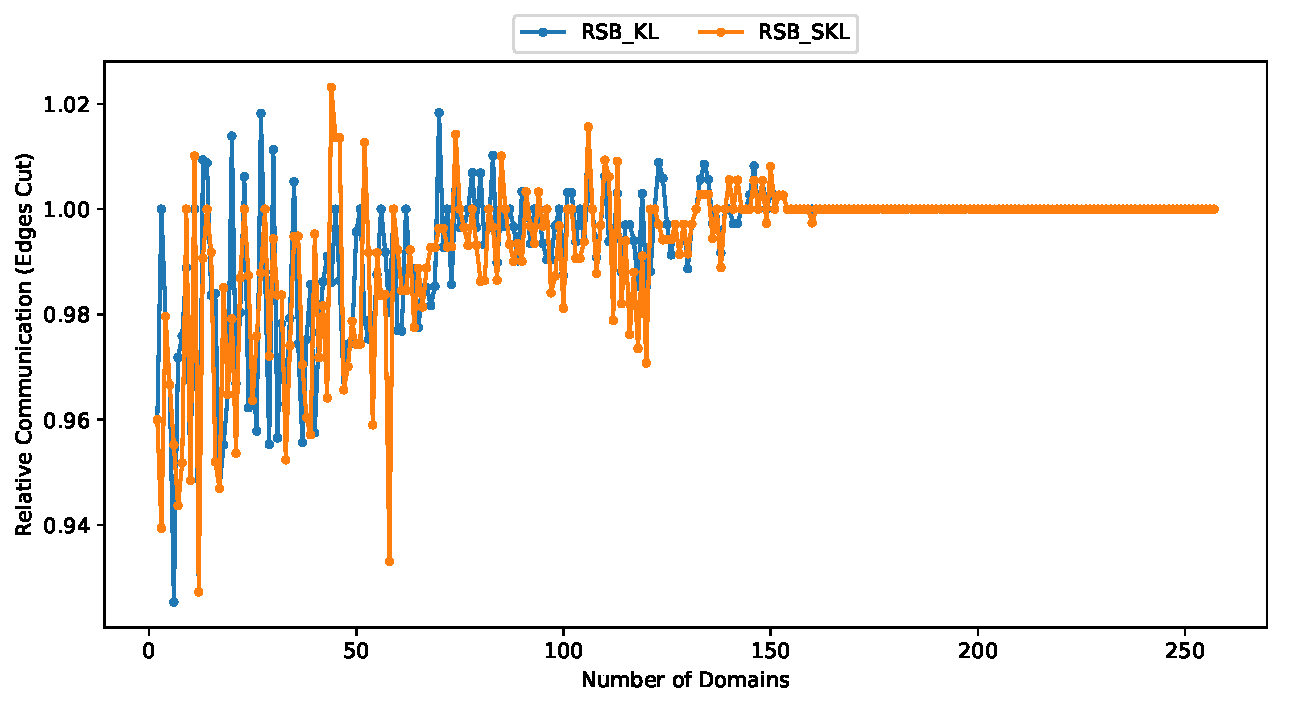
\includegraphics[width=\resultwidth]{results/2D/RSB_Edges_Cut_Relative}
        \caption{Communication relative to the \ac{RSB} method without refinement as a function of number of domains for each refinement method using the \ac{RSB} partitioning method.\label{fig:Spatial Decomposition:2D RSB Refinement}}
      \end{figure}

      \begin{figure}
        \centering
        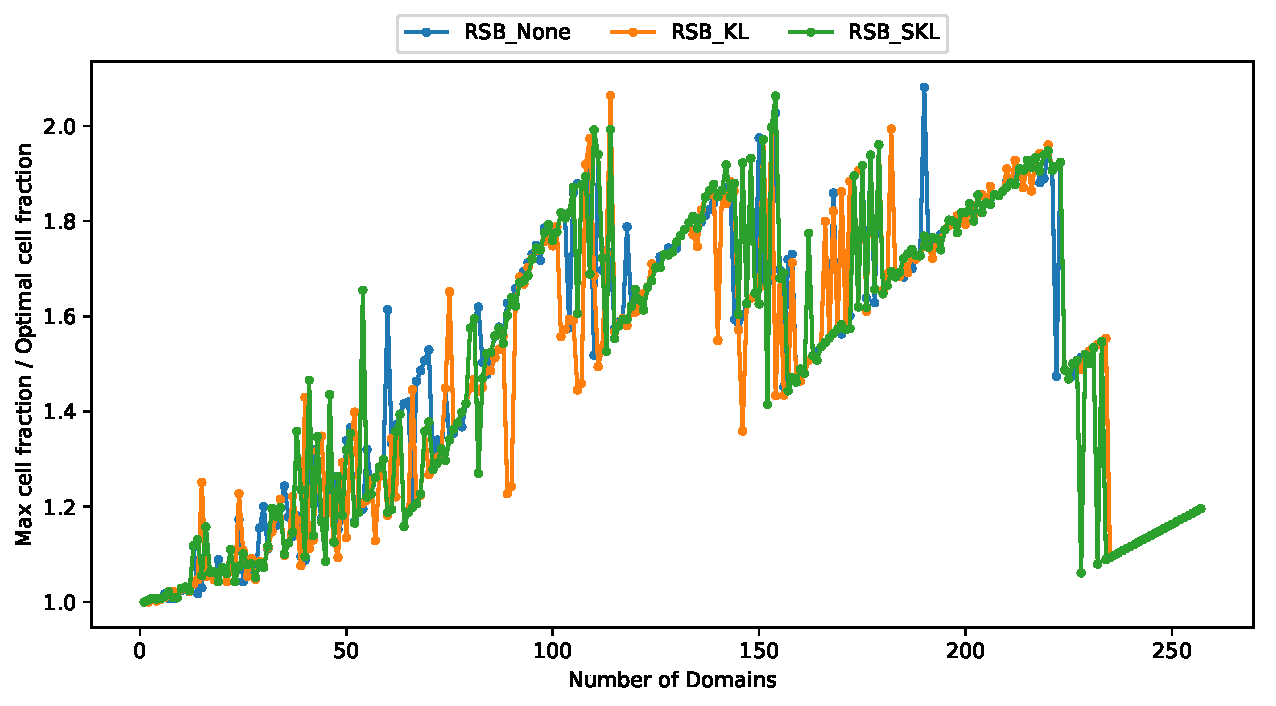
\includegraphics[width=\resultwidth]{results/2D/RSB_Size_to_Optimal}
        \caption{Ratio of maximum cell fraction to optimal cell fraction for the \ac{RSB} partitioning method with each refinement method. \label{fig:Spatial Decomposition:RSB Refinement Balance}}
      \end{figure}
    }
  }
  %%%%%%%%%%%%%%%%%%%%%%%%%%%%%%%%%%%%%%%%%%%%%%%%%%%%%%%%%%%%%%%%%%%%%%%%%%%%%%
  % Conclusions
  %%%%%%%%%%%%%%%%%%%%%%%%%%%%%%%%%%%%%%%%%%%%%%%%%%%%%%%%%%%%%%%%%%%%%%%%%%%%%%
  \section{Conclusions}{\label{sec:Spatial Decomposition:Conclusions}
    Spatial decomposition is a useful technique for reducing the runtime of simulations and is necessary to run whole-core high fidelity reactor calculations.
    Using graph partitioning methods to decompose the spatial domain of a core has significant advantages when compared to previous decomposition methods.
    Graph partitioning allows for the usage of an arbitrary number of spatial subdomains, and it generalizes to different module geometries such as a hexagonal lattice.
    Graph partitioning methods generally provide high quality decompositions that increase parallel efficiency.
    These automated spatial decomposition methods improve code usability and flexibility by allowing users to easily fit simulations to any number of processors.

    However, for highly decomposed cores, the convergence rate decreases due to jagged subdomain boundaries.
    This caused graph partitioning methods to significantly reduce runtime for problems that were not highly decomposed but actually increase runtime for highly decomposed problems.
    This is because the assembly-based decomposition method used rectangular (non-jagged) subdomains.
    This indicates that it may be advantageous to create a high quality decomposition method that enforces rectangular subdomains.
    However, this approach will not generalize to other lattice types, such as hexagonal lattices.

    In the current MPACT implementation, there is no significant difference in run-times when using any of the three partitioning methods discussed, although \ac{REB} typically results in slightly lower \ac{MOC} run-times.
    The 2-D results indicate that the maximum fraction of cells in a subdomain is highly correlated with the runtime of the simulation.
    Furthermore, 2-D results indicate that the parallel efficiency of \ac{MOC} is highly correlated with the ratio of the optimal cell fraction per subdomain to the maximum cell fraction in a subdomain.

    In 3-D, MPACT currently requires spatial domains to be axially and radially aligned.
    If these restrictions are lifted, then other approaches can be used to perform the 3-D spatial decomposition.
    Three 3-D decomposition approaches were investigated in this work: radial and axial aligned subdomains, radially aligned subdomains, and an approach with no alignment restrictions.
    The radially aligned approach is expected to out perform the current approach by an average of 10\% for typical cases.
    However, the unrestricted approach is actually expected to perform worse than the current approach on average.
    This analysis was performed on a 3-D core, which was relatively homogeneous in the axial direction; if a core design were to be more axially heterogeneous, then a more significant increase in performance might be expected.

    The parallel efficiency is a measure of how well computational resources are utilized in parallel applications.
    MPACT's overall parallel efficiency decreases rapidly as more domains are used due to two factors: increased number of iterations, and the inefficiency of parallel \ac{CMFD} solves.
    For the 2-D VERA progression problem 5a, the overall parallel efficiency of MPACT dropped to nearly 20\%.
    The parallel efficiency of only the \ac{MOC} computations in MPACT drops to between 40--60\%, while the parallel efficiency of the \ac{CMFD} computation drops to $<\!\!20$\%.
    This causes the \ac{CMFD} computation to dominate runtime in spatially decomposed cases, and motivates the implementation of a more efficient parallel linear system operator in MPACT rather than using a third-party library.
  }

  % References
  \printbibliography
}